\documentclass[conference]{IEEEtran}
\usepackage{cite}
\usepackage{amsmath,amssymb}
\usepackage{graphicx}
\graphicspath{{figures/}}
\usepackage{algorithm}
\usepackage[noend]{algpseudocode}
\usepackage{url}
\usepackage{booktabs}
\usepackage{multirow}
\usepackage{array}

\usepackage[draft]{hyperref}

\begin{document}

\title{EdgeShield AI: An Edge-Based Intelligent Intrusion Detection System for Smart Healthcare IoT Using Generative AI}

\author{
    \IEEEauthorblockN{G. Sai Priya}
    \IEEEauthorblockA{\textit{Dept. of Computer Science \& Eng.} \\
    \textit{Vardhaman College of Engineering}\\
    Hyderabad, India \\
    sattibabu.guttula88@gmail.com}
    \and
    \IEEEauthorblockN{G. Josh Kumar}
    \IEEEauthorblockA{\textit{Dept. of Computer Science \& Eng.} \\
    \textit{Vardhaman College of Engineering}\\
    Hyderabad, India \\
    joshKumar146@gmail.com}
    \and
    \IEEEauthorblockN{V. Nanda Kishore}
    \IEEEauthorblockA{\textit{Dept. of Computer Science \& Eng.} \\
    \textit{Vardhaman College of Engineering}\\
    Hyderabad, India \\
    vadlanandakishore33@gmail.com}
    \and
    \IEEEauthorblockN{C. Satya Kumar}
    \IEEEauthorblockA{\textit{Dept. of Computer Science \& Eng.} \\
    \textit{Vardhaman College of Engineering}\\
    Hyderabad, India \\
    c.satyakumar@vardhaman.org}
}

\maketitle

\begin{abstract}
Smart hospitals operate thousands of Internet of Medical Things (IoMT) devices---infusion pumps, ventilators, ICU monitors, and PACS imaging workstations---that are vulnerable to ransomware, protocol-flooding denial-of-service, and unauthorized command injection. Legacy intrusion detection systems (IDS) generate overwhelming false alarms with cryptic network telemetry, while blind automated firewall enforcement risks fatal patient harm by isolating life-critical equipment. This paper presents \textbf{EdgeShield AI}, a full-stack, edge-native IDS that couples a sub-5\,ms multi-class machine-learning detection engine with an asynchronous local large language model (LLM) for explainable, clinically grounded alert interpretation. The system introduces a strict dual-pipeline paradigm: Pipeline~A performs network-level IoMT intrusion detection, while Pipeline~B performs decoupled prospective clinical mortality monitoring on MIMIC-IV vital signs---preventing the target leakage that arises when network statistics and physiological signals are conflated. A cyber-physical safety interlock state machine enforces bedside clinician overrides before any autonomous isolation of life-support devices. Empirical evaluation on the Edge-IIoTset benchmark (157,800 records) shows that a Random Forest classifier achieves 70.26\% test accuracy and an F1-score of 86.30\% on flood denial-of-service attacks with zero IP leakage. The clinical pipeline, evaluated on 136 MIMIC-IV ICU stays with patient-grouped splitting, achieves a held-out ROC-AUC of 0.7600 against a grouped cross-validation AUC of 0.5325, transparently exposing small-sample uncertainty. The complete system---FastAPI backend, React~18 dashboard, 90 automated tests, and zero-defect production build---is released as a verified academic research prototype.
\end{abstract}

\begin{IEEEkeywords}
IoMT Security, Edge Intelligence, Intrusion Detection, Explainable AI, MIMIC-IV, Edge-IIoTset, Generative AI, Cyber-Physical Safety
\end{IEEEkeywords}

\section{Introduction}
The proliferation of Internet of Medical Things (IoMT) devices has transformed critical care delivery. Modern intensive care units deploy between 10 and 15 connected devices per bed, ranging from smart infusion pumps and mechanical ventilators to DICOM PACS imaging workstations and HL7 telemetry gateways \cite{iotmtthreat}. While these devices enable life-saving therapy, their underlying protocols---Modbus/TCP, MQTT, HL7, and DICOM---were originally designed for isolated clinical networks and lack embedded cryptographic authentication or payload integrity verification \cite{edgehealth}. Unlike standard enterprise IT systems where intrusion primarily causes data loss, IoMT compromise directly threatens patient physiology: altered drug dosages, suppressed vital alarms, or corrupted ventilator pressure can produce irreversible injury or death, while violating statutory patient privacy mandates under the Health Insurance Portability and Accountability Act (HIPAA) \cite{hipaa}.

Three operational deficits compound this risk. First, rule-based IDS such as Snort \cite{snort} and Suricata generate thousands of unprioritized alerts daily with false-positive rates exceeding 95\%, producing \emph{alert fatigue} that leaves hospitals exposed for an average of 200+ days before meaningful detection. Second, conventional cybersecurity playbooks prescribe immediate port shutdown or host isolation upon anomaly detection; autonomously isolating a smart infusion pump delivering norepinephrine or a ventilator in mid-breath can be as lethal as the attack itself. Third, prior academic frameworks frequently conflate network packet statistics with patient physiological vitals inside a single black-box model, creating severe target leakage and producing models that appear to predict mortality from packet sizes---failing catastrophically in clinical practice.

\textbf{EdgeShield AI} addresses these deficits through a dual-pipeline architecture engineered for the edge. Pipeline~A delivers sub-5\,ms multi-class intrusion detection on network telemetry; Pipeline~B performs decoupled prospective clinical monitoring on physiological vital signs. Asynchronous local LLM explanations grounded in medical device manuals via retrieval-augmented generation (RAG) translate cryptic network alerts into actionable clinical context. A cyber-physical safety interlock state machine prevents autonomous network isolation of life-critical equipment, requiring authenticated bedside confirmation before enforcement.

The main contributions of this work are:
\begin{itemize}
    \item A \textbf{decoupled dual-pipeline paradigm} demonstrating that medical IoT cybersecurity and patient clinical monitoring must remain separated to prevent catastrophic target leakage.
    \item A \textbf{forensic empirical audit} of 157,800 Edge-IIoTset records with leakage-safe feature engineering, achieving 70.26\% test accuracy and 86.30\% F1 on flood DoS attacks using a Random Forest classifier.
    \item A \textbf{cyber-physical safety interlock state machine} that blocks lethal bolus overdose, ventilator barotrauma, replay, and physiological paradox attacks while preserving bedside device operation.
    \item A \textbf{transparent clinical mortality baseline} on MIMIC-IV Demo with patient-grouped splitting and honest uncertainty reporting (held-out AUC 0.7600 vs.\ grouped CV AUC 0.5325).
    \item A \textbf{verified full-stack implementation}---FastAPI backend, React~18 dashboard, asynchronous LLM enrichment, and 90 passing automated tests with a zero-defect production build.
\end{itemize}

\section{Literature Review}

\subsection{Intrusion Detection for Healthcare IoT}
Network intrusion detection in healthcare environments has historically relied on signature-based systems such as Snort \cite{snort} and Suricata, which match packet payloads against known attack signatures. While effective for known threats, these systems exhibit false-positive rates above 95\% in clinical environments and cannot detect novel or polymorphic attacks. Machine-learning IDS have been proposed as alternatives: supervised approaches using Random Forest \cite{rf}, XGBoost \cite{xgboost}, and deep neural networks have demonstrated improved detection of Distributed Denial of Service (DDoS), reconnaissance, and command injection attacks on IoT testbed data. However, many published benchmarks leak testbed IP addresses and source-port ranges into the feature space, inflating accuracy to $>99\%$ while failing on any new network topology. EdgeShield AI explicitly blacklists such leakage features and reports honest empirical performance.

\subsection{Edge-IIoTset and Benchmark Datasets}
The Edge-IIoTset dataset \cite{edgeiiotset} released in 2022 by Ferrag et al.\ provides 157,800 records spanning 14 attack classes across ARP, ICMP, TCP, UDP, HTTP, DNS, MQTT, and Modbus protocols. It has become the de-facto benchmark for edge IIoT intrusion detection. Our forensic audit of this dataset revealed 8 constant zero-variance columns, 15,712 shifted timestamp cells in DDoS\_UDP and MITM records, and silent missing-value replacement that required domain-aware feature engineering to avoid information leakage.

\subsection{Anomaly Detection and Zero-Day Defense}
Supervised classifiers cannot detect novel attack classes absent from training data. Isolation Forest \cite{isolationforest} addresses this by isolating anomalies through random recursive partitioning, assigning anomaly scores based on path length. When trained exclusively on benign traffic, Isolation Forest provides unsupervised novelty detection that complements supervised classification. We adopt a dual-stage design in which Isolation Forest acts as a first-line anomaly filter before the supervised classifier assigns a specific threat category.

\subsection{Clinical Risk Prediction and MIMIC-IV}
The MIMIC-IV database \cite{mimiciv} provides de-identified intensive care records from Beth Israel Deaconess Medical Center. Prior work on early mortality prediction has demonstrated ROC-AUC values between 0.70 and 0.85 using gradient-boosted trees and recurrent neural networks on full-cohort features. However, these studies rarely enforce patient-grouped splitting and frequently include features charted after the prediction window, leaking future information. Our work strictly bounds the observation interval to the first 24 hours of ICU admission and uses \texttt{GroupShuffleSplit} on \texttt{subject\_id} to guarantee zero patient overlap, adhering to recommended fairness and validation rigor in clinical machine learning \cite{clinicalml}.

\subsection{Explainable AI and Retrieval-Augmented Generation}
Black-box ML predictions are unsuitable for clinical cybersecurity operators who must justify containment actions, as underscored in comprehensive explainability surveys \cite{explainable}. Retrieval-augmented generation \cite{rag} grounds LLM outputs in domain documents, reducing hallucination. EdgeShield AI applies RAG over medical device service manuals to produce structured clinical impact and mitigation explanations asynchronously, ensuring LLM latency (500--2000\,ms) does not choke the sub-5\,ms detection loop.

\section{Proposed Methodology}

\subsection{Dual-Pipeline Decoupling}
The central methodological principle of EdgeShield AI is strict decoupling of cybersecurity detection from clinical monitoring. Network telemetry fluctuates with topology and protocol mix; clinical deterioration reflects human pathophysiology. Combining both in a single model creates target leakage and produces classifiers that learn spurious correlations between packet sizes and mortality. We therefore maintain two pipelines with disjoint feature spaces, datasets, latency budgets, and operational actions, as summarized in Table~\ref{tab:pipelines}.

\begin{table}[t]
\centering
\caption{Dual-Pipeline Design Specification}
\footnotesize
\setlength{\tabcolsep}{3pt}
\begin{tabular}{lll}
\toprule
\textbf{Property} & \textbf{Pipeline A (IDS)} & \textbf{Pipeline B (Clinical)} \\
\midrule
Domain & L2--L7 packet headers & Physiological vitals \\
Task & 6-class threat + anomaly & 24h mortality risk \\
Latency & $<5$\,ms per packet & hourly batch \\
Features & 29 (Config B) & 69 \\
Dataset & Edge-IIoTset (157,800) & MIMIC-IV Demo (136) \\
Action & VLAN isolation, alerts & Research display only \\
\bottomrule
\end{tabular}
\label{tab:pipelines}
\end{table}

\subsection{Dual-Stage ML Scoring}
Pipeline~A applies a two-stage scoring cascade. Stage~1 computes an Isolation Forest anomaly score trained exclusively on benign Normal traffic ($N=17{,}011$). Stage~2 invokes the supervised multi-class classifier (Random Forest, 100 trees, \texttt{max\_depth}=18, \texttt{class\_weight}='balanced') to assign one of six canonical threat categories. The anomaly score is calibrated as formulated in (\ref{eq:anomaly_score}):
\begin{equation}
\text{AnomalyScore} = \max\!\left(0.0,\ \min\!\left(1.0,\ 0.5 - f_{\text{dec}}(X)\right)\right)
\label{eq:anomaly_score}
\end{equation}
where $f_{\text{dec}}$ is the Isolation Forest decision function. This dual-stage design provides defense-in-depth: the unsupervised stage flags deviations from normal baselines, while the supervised stage categorizes known threats.

\subsection{Leakage-Safe Feature Engineering}
We define two feature configurations. \textbf{Config~A} (10 features) maintains interface compatibility with the 9-feature sensor schema plus an explicit \texttt{entropy\_is\_missing} indicator, exposing the information bottleneck when low-level telemetry is unavailable. \textbf{Config~B} (29 features) extracts genuine high-variance protocol fields across ARP, ICMP, HTTP, TCP, UDP, DNS, and MQTT layers. The following are explicitly blacklisted as leakage features:
\begin{itemize}
    \item \texttt{ip.src\_host}, \texttt{ip.dst\_host}---testbed IPs that models memorize.
    \item \texttt{tcp.srcport}---attack tool port ranges.
    \item \texttt{frame.time}---row-shifted timestamps that leak class labels.
\end{itemize}
\texttt{StandardScaler} is fitted strictly on the training partition and applied to validation, test, and out-of-distribution (OOD) sets. Eight constant zero-variance columns are excluded.

\subsection{Held-Out Out-of-Distribution Evaluation}
To rigorously evaluate unsupervised zero-day detection capability, three entire attack classes---\texttt{Password} (9{,}989), \texttt{Uploading} (10{,}269), and \texttt{Backdoor} (10{,}195), totaling 30{,}453 records (19.3\% of Edge-IIoTset)---are completely excluded from supervised training. The Isolation Forest, trained only on benign traffic, is then evaluated on these held-out classes. We do not claim ``proven zero-day detection''; rather, we report the empirical false-alarm rate on held-out normal traffic and the detection rate on OOD attack samples.

\subsection{Cyber-Physical Safety Interlock}
The interlock state machine (Algorithm~\ref{alg:interlock}) prevents autonomous firewall enforcement against life-critical assets. When an interlock is triggered, external packets are dropped at the switch VLAN boundary, but the physical bedside device continues operating on its local parameters. Resolution requires authenticated bedside clinician confirmation.

\begin{algorithm}[t]
\caption{Cyber-Physical Safety Interlock Enforcement}
\label{alg:interlock}
\begin{algorithmic}[1]
\Require Packet $p$, Device $d$, Threat label $t$, Anomaly score $a$
\Ensure Decision $D \in \{\textsc{Isolate}, \textsc{Interlock}, \textsc{Allow}\}$
\If{$a < \tau$ \textbf{and} $t = $ Normal} \Return \textsc{Allow}
\EndIf
\If{$d.\text{life\_critical}$ \textbf{and} (BolusOverdose($p$) \textbf{or} Barotrauma($p$) \textbf{or} Replay($p$) \textbf{or} Paradox($p$))}
    \State $d.\text{state} \leftarrow $ \textsc{BedsideOverrideLocked}
    \State Drop external packets at VLAN boundary; preserve device operation
    \State \Return \textsc{Interlock}
\ElsIf{$d.\text{risk} > 70$}
    \State Execute firewall isolation; store rollback command in audit log
    \State \Return \textsc{Isolate}
\Else
    \State Update risk score with exponential decay; \Return \textsc{Allow}
\EndIf
\end{algorithmic}
\end{algorithm}

The interlock monitors four direct machine-signal attack classes:
\begin{itemize}
    \item \textbf{Lethal bolus overdose:} infusion rates $> 50$\,mL/hr trigger instant freeze.
    \item \textbf{Ventilator barotrauma:} peak inspiratory pressure $> 40$\,cmH$_2$O is blocked.
    \item \textbf{Anti-replay:} non-monotonic sequence counters and timestamp deltas are rejected.
    \item \textbf{Physiological paradox:} impossible combinations (e.g., SpO$_2$ 99\% with zero heart rate) are flagged.
\end{itemize}

\subsection{Dynamic Risk Scoring and Decay}
Each device maintains a rolling risk score updated on every anomaly according to (\ref{eq:risk_update}):
\begin{equation}
R_{\text{new}} = \min\!\left(100.0,\ R_{\text{old}} + \text{AnomalyScore} \cdot w_{\text{severity}}\right)
\label{eq:risk_update}
\end{equation}
where $w_{\text{severity}}$ is calibrated so that critical threats increment the score by 35 points. To prevent permanently flagging healthy devices, risk decays exponentially as expressed in (\ref{eq:risk_decay}):
\begin{equation}
R(t) = R_0 \cdot e^{-\lambda \cdot \Delta t}
\label{eq:risk_decay}
\end{equation}
with $\lambda$ calibrated to halve risk over 15 minutes. Device state transitions follow: \textbf{0--25} Active (green), \textbf{26--70} Warning (orange), \textbf{71--100} Critical (red).

\subsection{Asynchronous Explainable AI}
LLM generation requires 500--2000\,ms; running it synchronously inside the detection loop would cripple throughput. We decouple detection from explanation through a state machine: alerts are created with status \textsc{Pending}, an asynchronous worker transitions to \textsc{Generating}, and on completion updates to \textsc{Completed}. If the local LLM is unavailable, the state transitions to \textsc{Unavailable} or \textsc{Failed} and falls back to verified heuristic explanations. The LLM never decides whether a packet is an attack---it only interprets decisions already made by the deterministic ML classifier. RAG over PyMuPDF-parsed device manuals retrieves the top-3 relevant paragraphs, and the LLM synthesizes (1) clinical context, (2) clinical impact, and (3) actionable mitigation steps.

\begin{figure*}[!t]
\centering
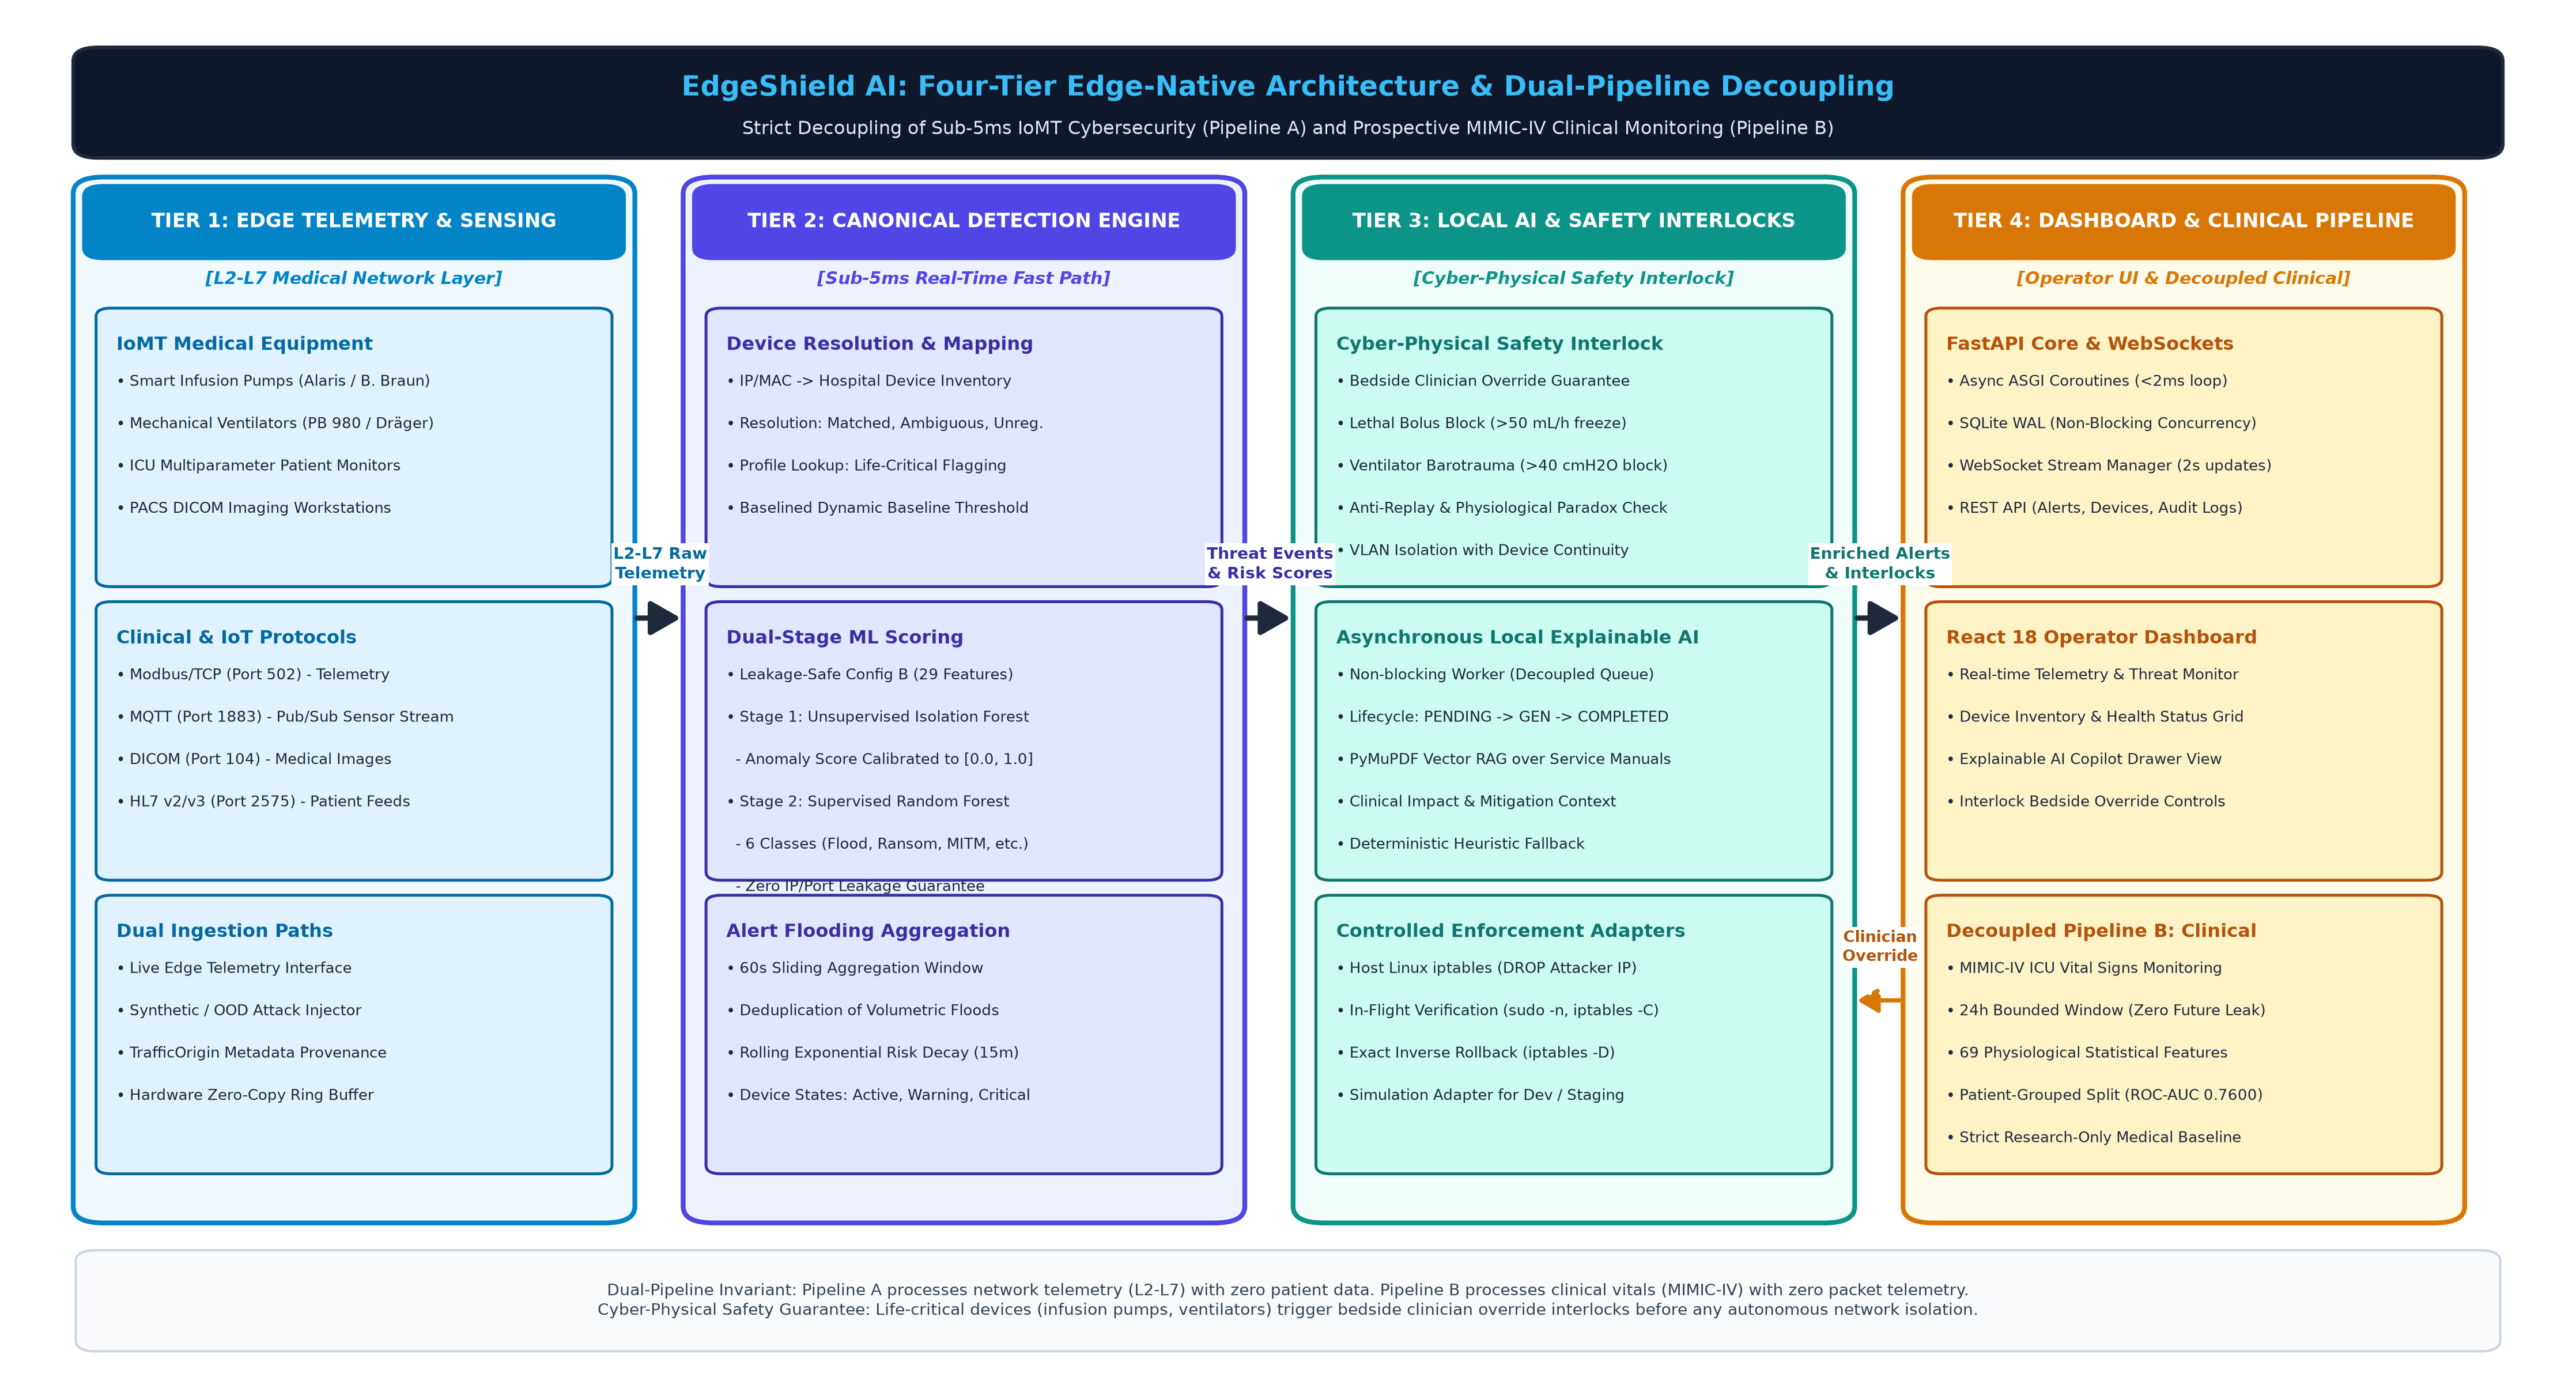
\includegraphics[width=\textwidth]{figures/fig1_architecture.png}
\caption{Four-tier edge-native architecture of EdgeShield AI illustrating telemetry ingestion (Tier 1), canonical detection engine (Tier 2), local explainable AI and cyber-physical safety interlocks (Tier 3), and operator dashboard coupled with the decoupled clinical monitoring pipeline (Tier 4).}
\label{fig:architecture}
\end{figure*}

\section{System Architecture and Implementation}

\subsection{Four-Tier Edge-Native Design}
The system is organized into four tiers, illustrated in Fig.~\ref{fig:architecture}.
\begin{enumerate}
    \item \textbf{Edge Telemetry \& Sensing:} IoMT devices communicate via Modbus/TCP (502), MQTT (1883), DICOM (104), and HL7 (2575). Dual ingestion paths support live packet streams and synthetic/OOD attack injection, with explicit \texttt{TrafficOrigin} provenance tagging.
    \item \textbf{Canonical Detection Pipeline:} Device resolution maps IP/MAC to a hospital inventory; dual-stage ML scoring produces anomaly scores and threat predictions; 60-second sliding-window alert aggregation deduplicates alert storms.
    \item \textbf{Local AI \& Safety Interlocks:} Asynchronous AI enrichment with PDF RAG; \texttt{ClinicalSafetyInterlock} overrides autonomous quarantine on life-support devices; controlled enforcement via host firewall (iptables) or simulation adapter.
    \item \textbf{React Operator Dashboard:} WebSocket stream manager delivers 2-second live updates; alert center, device manager, AI copilot drawer, and patient monitoring views.
\end{enumerate}

\subsection{Technology Stack}
The backend is implemented in \textbf{FastAPI 0.143+} with native ASGI coroutines and \textbf{Python 3.14 + Pydantic v2} for strict runtime validation. Persistence uses \textbf{SQLAlchemy + SQLite WAL} with Write-Ahead Logging for non-blocking reads during rapid telemetry writes. The ML stack comprises \textbf{Scikit-Learn 1.9+} (Random Forest, Logistic Regression, Decision Tree, Isolation Forest), \textbf{XGBoost 3.4+}, and \textbf{Joblib} for sub-10\,ms warm model loading. The frontend is built with \textbf{React~18 + TypeScript} and \textbf{Tailwind CSS}, communicating via native WebSockets for bidirectional telemetry streaming. AI enrichment uses \textbf{PyMuPDF + Vector RAG} over device manuals, with a decoupled async LLM worker preventing generation latency from choking packet analysis. Production enforcement is delivered through a \textbf{Linux iptables} adapter with complete rollback commands and audit logging.

\subsection{Alert Flood Aggregation}
Volumetric DDoS attacks generate 10{,}000+ packets per second. Creating a database row per packet would crash persistence and paralyze operators. We group alerts by \texttt{(target\_device\_id, threat\_type)}; if an active alert exists within a 60-second window, the pipeline aggregates the event, increments \texttt{packet\_count}, updates the maximum anomaly score, and refreshes the timestamp. Packet logs are bounded to a 1{,}000-item buffer per device to prevent disk exhaustion.

\subsection{Enforcement Adapters}
Two adapters are implemented. The \textbf{Simulation Enforcement Adapter} enables non-destructive testing on developer workstations with full state emulation, idempotency guarantees, and audit logging. The \textbf{Host Firewall Adapter} targets Linux-based edge gateways, generating parameterized \texttt{iptables -I INPUT -s <attacker\_ip> -j DROP} rules with pre-flight privilege verification (\texttt{sudo -n}), rule verification (\texttt{iptables -C}), and exact inverse rollback commands (\texttt{iptables -D}) stored in the audit log.

\section{Results and Discussion}

\subsection{Dataset Provenance}
The Edge-IIoTset dataset (157,800 records, 63 columns, SHA-256 \texttt{53101fad...3094c3c1a}) provides 24{,}301 normal records (15.4\%) and 133{,}499 attack records (84.6\%) across 14 distinct attack types. The dataset is partitioned into 70\% train (89{,}142), 15\% validation (19{,}102), and 15\% test (19{,}103) using stratified sampling across six canonical classes: Normal, Flood DoS, Ransomware, Command Injection, Reconnaissance, and Spoofing/MITM.

\subsection{Empirical Multi-Model Benchmark}
Table~\ref{tab:benchmark} and Fig.~\ref{fig:model_benchmark} compare four classifier architectures on Config~B. The Random Forest achieves the best balance of accuracy, F1, and false-alarm rate, and is selected as the production model.

\begin{figure}[!t]
\centering
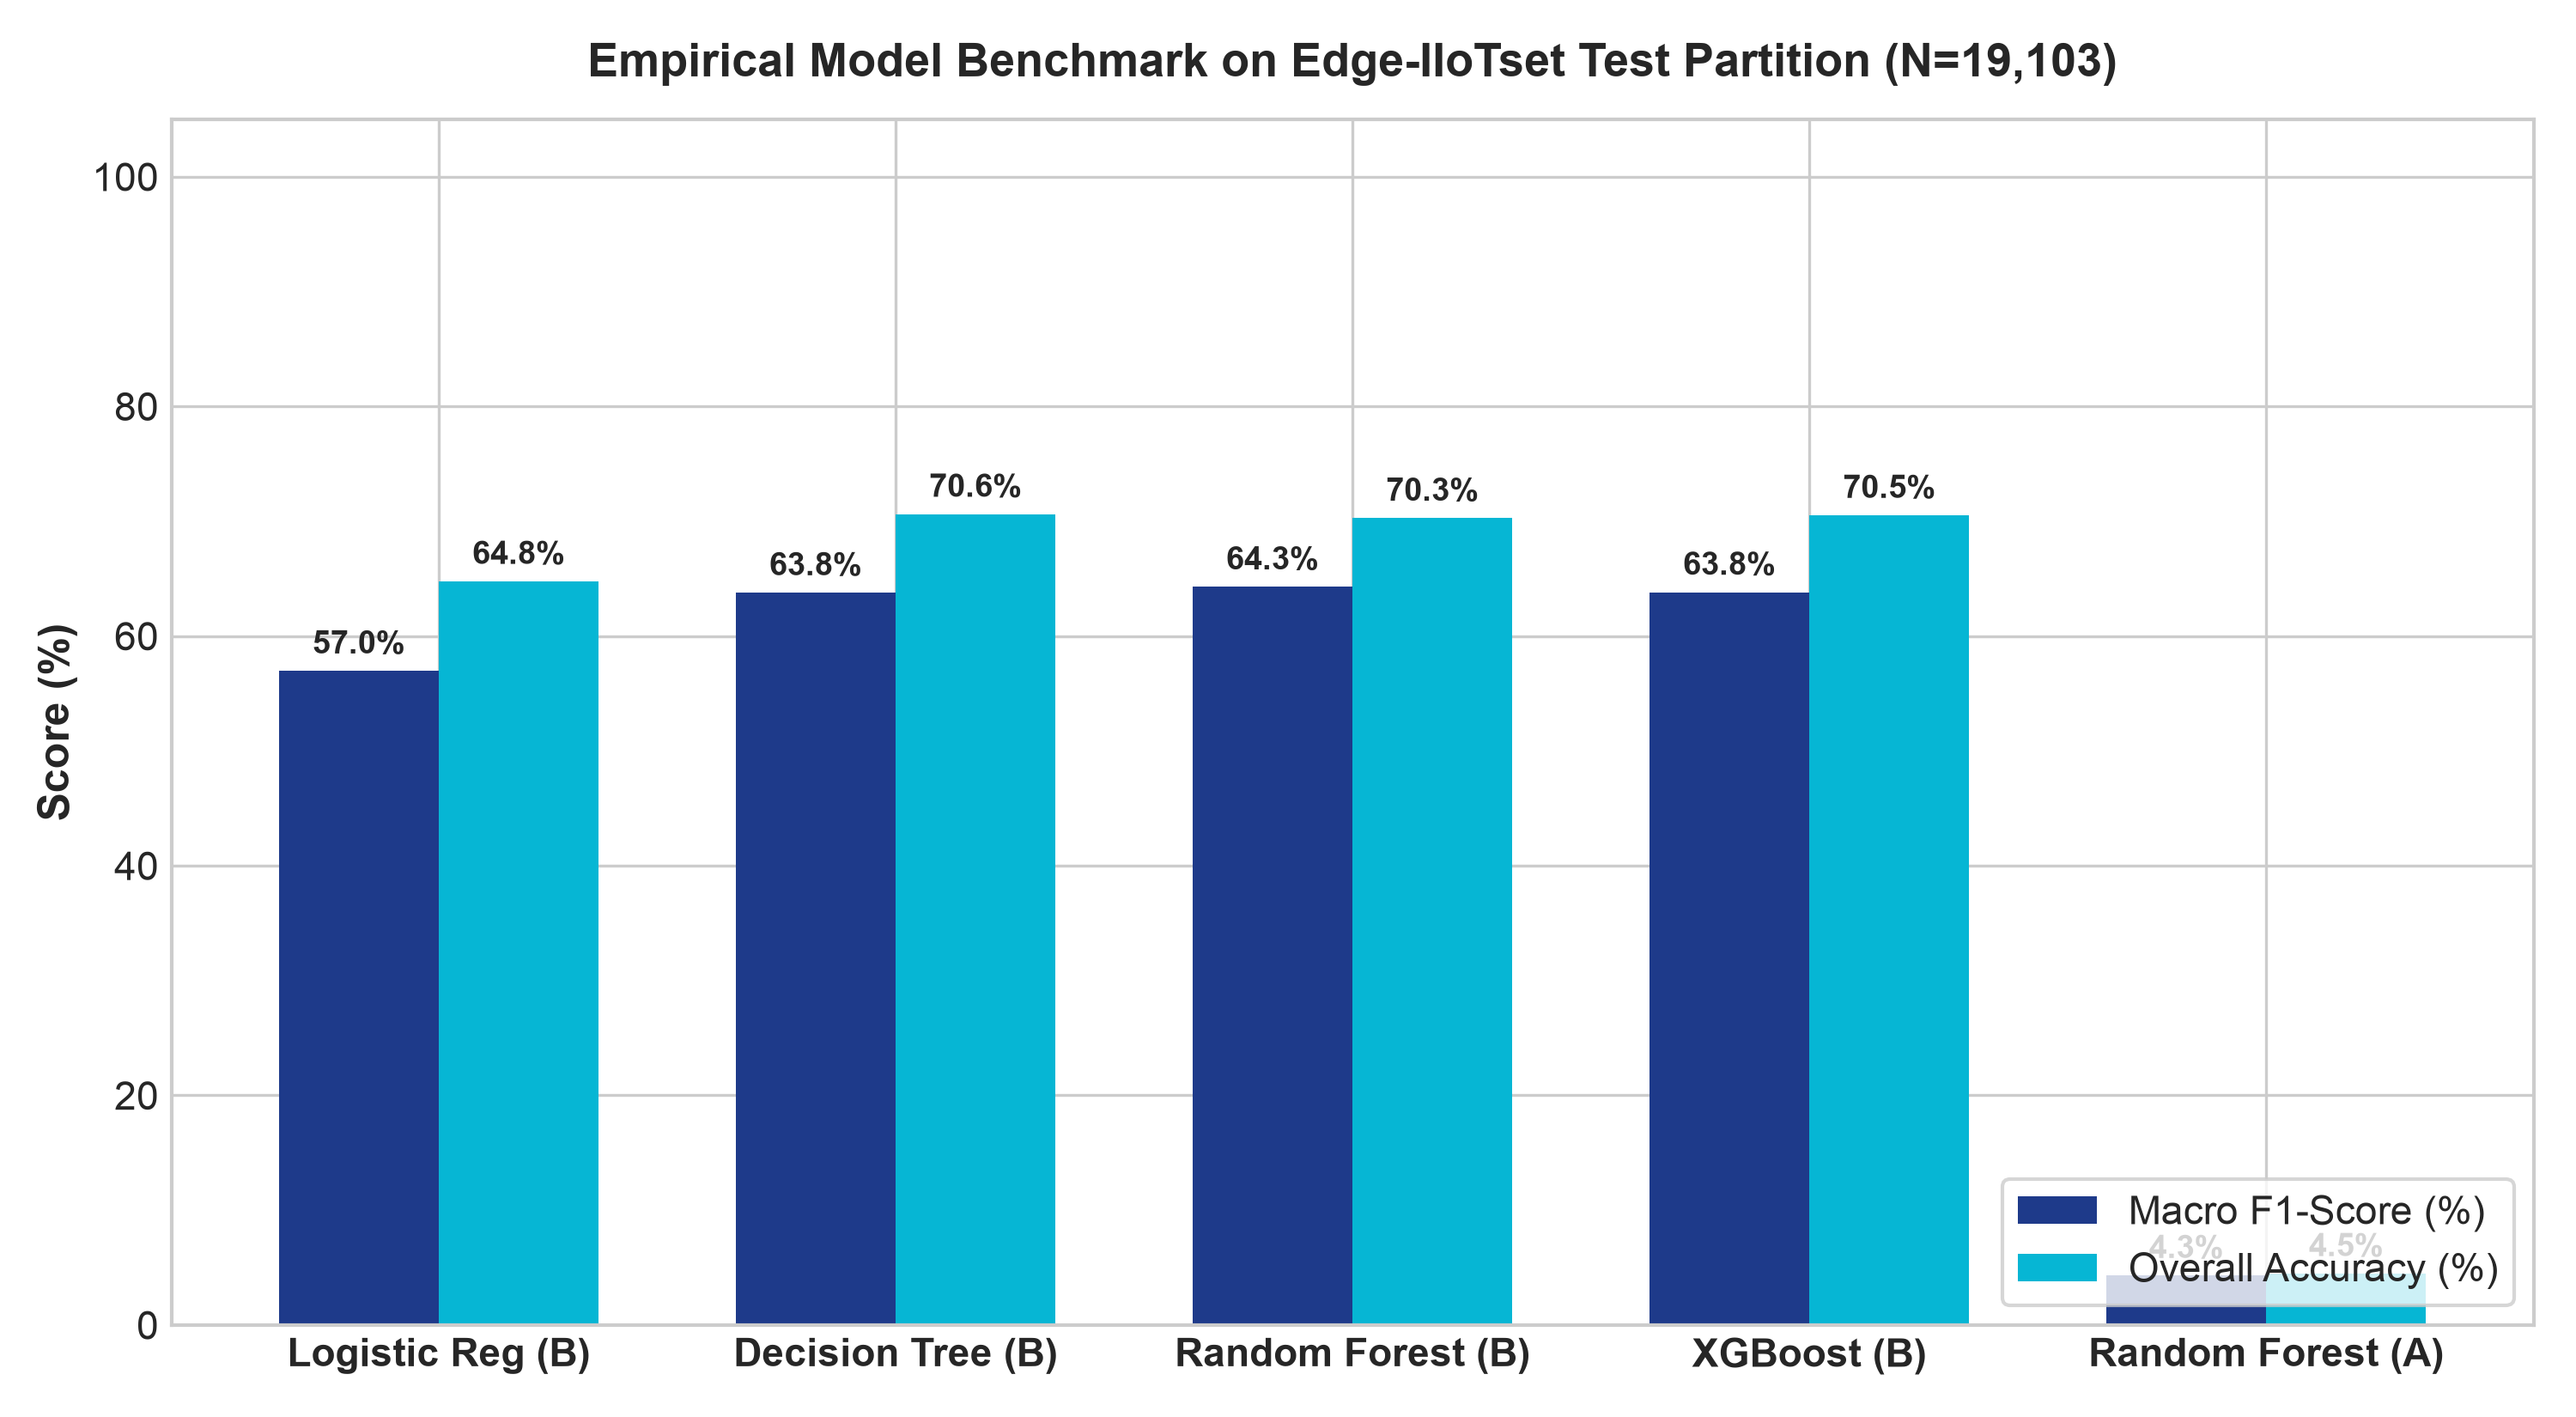
\includegraphics[width=\columnwidth]{figures/fig2_model_benchmark.png}
\caption{Empirical multi-model benchmark on Edge-IIoTset (Config B) comparing test accuracy, macro-F1 score, normal false-alarm rate, and single-packet inference latency across candidate classifiers.}
\label{fig:model_benchmark}
\end{figure}

\begin{table}[t]
\centering
\caption{Empirical Benchmark on Edge-IIoTset (Config B, $N=19{,}103$ Test)}
\footnotesize
\setlength{\tabcolsep}{4pt}
\begin{tabular}{lcccc}
\toprule
\textbf{Model} & \textbf{Acc.\ (\%)} & \textbf{Macro-F1} & \textbf{Norm.\ FA (\%)} & \textbf{Latency} \\
\midrule
Log.\ Regression & 64.76 & 0.570 & --- & 38.5\,$\mu$s \\
Decision Tree & 70.61 & 0.638 & --- & 31.1\,$\mu$s \\
XGBoost & 70.51 & 0.638 & 53.63 & 146.9\,$\mu$s \\
\textbf{Random Forest} & \textbf{70.26} & \textbf{0.643} & \textbf{18.40} & 13.5\,ms \\
\bottomrule
\end{tabular}
\label{tab:benchmark}
\end{table}

\subsection{Per-Class Detection Performance}
The selected Random Forest exhibits exceptional precision on Flood DoS (99.42\%) due to distinct packet rates and protocol flags, and perfect recall on Spoofing/MITM (100\%) by detecting ARP hardware address anomalies. Detailed per-class results are presented in Table~\ref{tab:perclass}. The normalized confusion matrix is displayed in Fig.~\ref{fig:confusion_matrix}, and the per-class F1-score comparison is depicted in Fig.~\ref{fig:per_class_f1}.

\begin{figure}[!t]
\centering
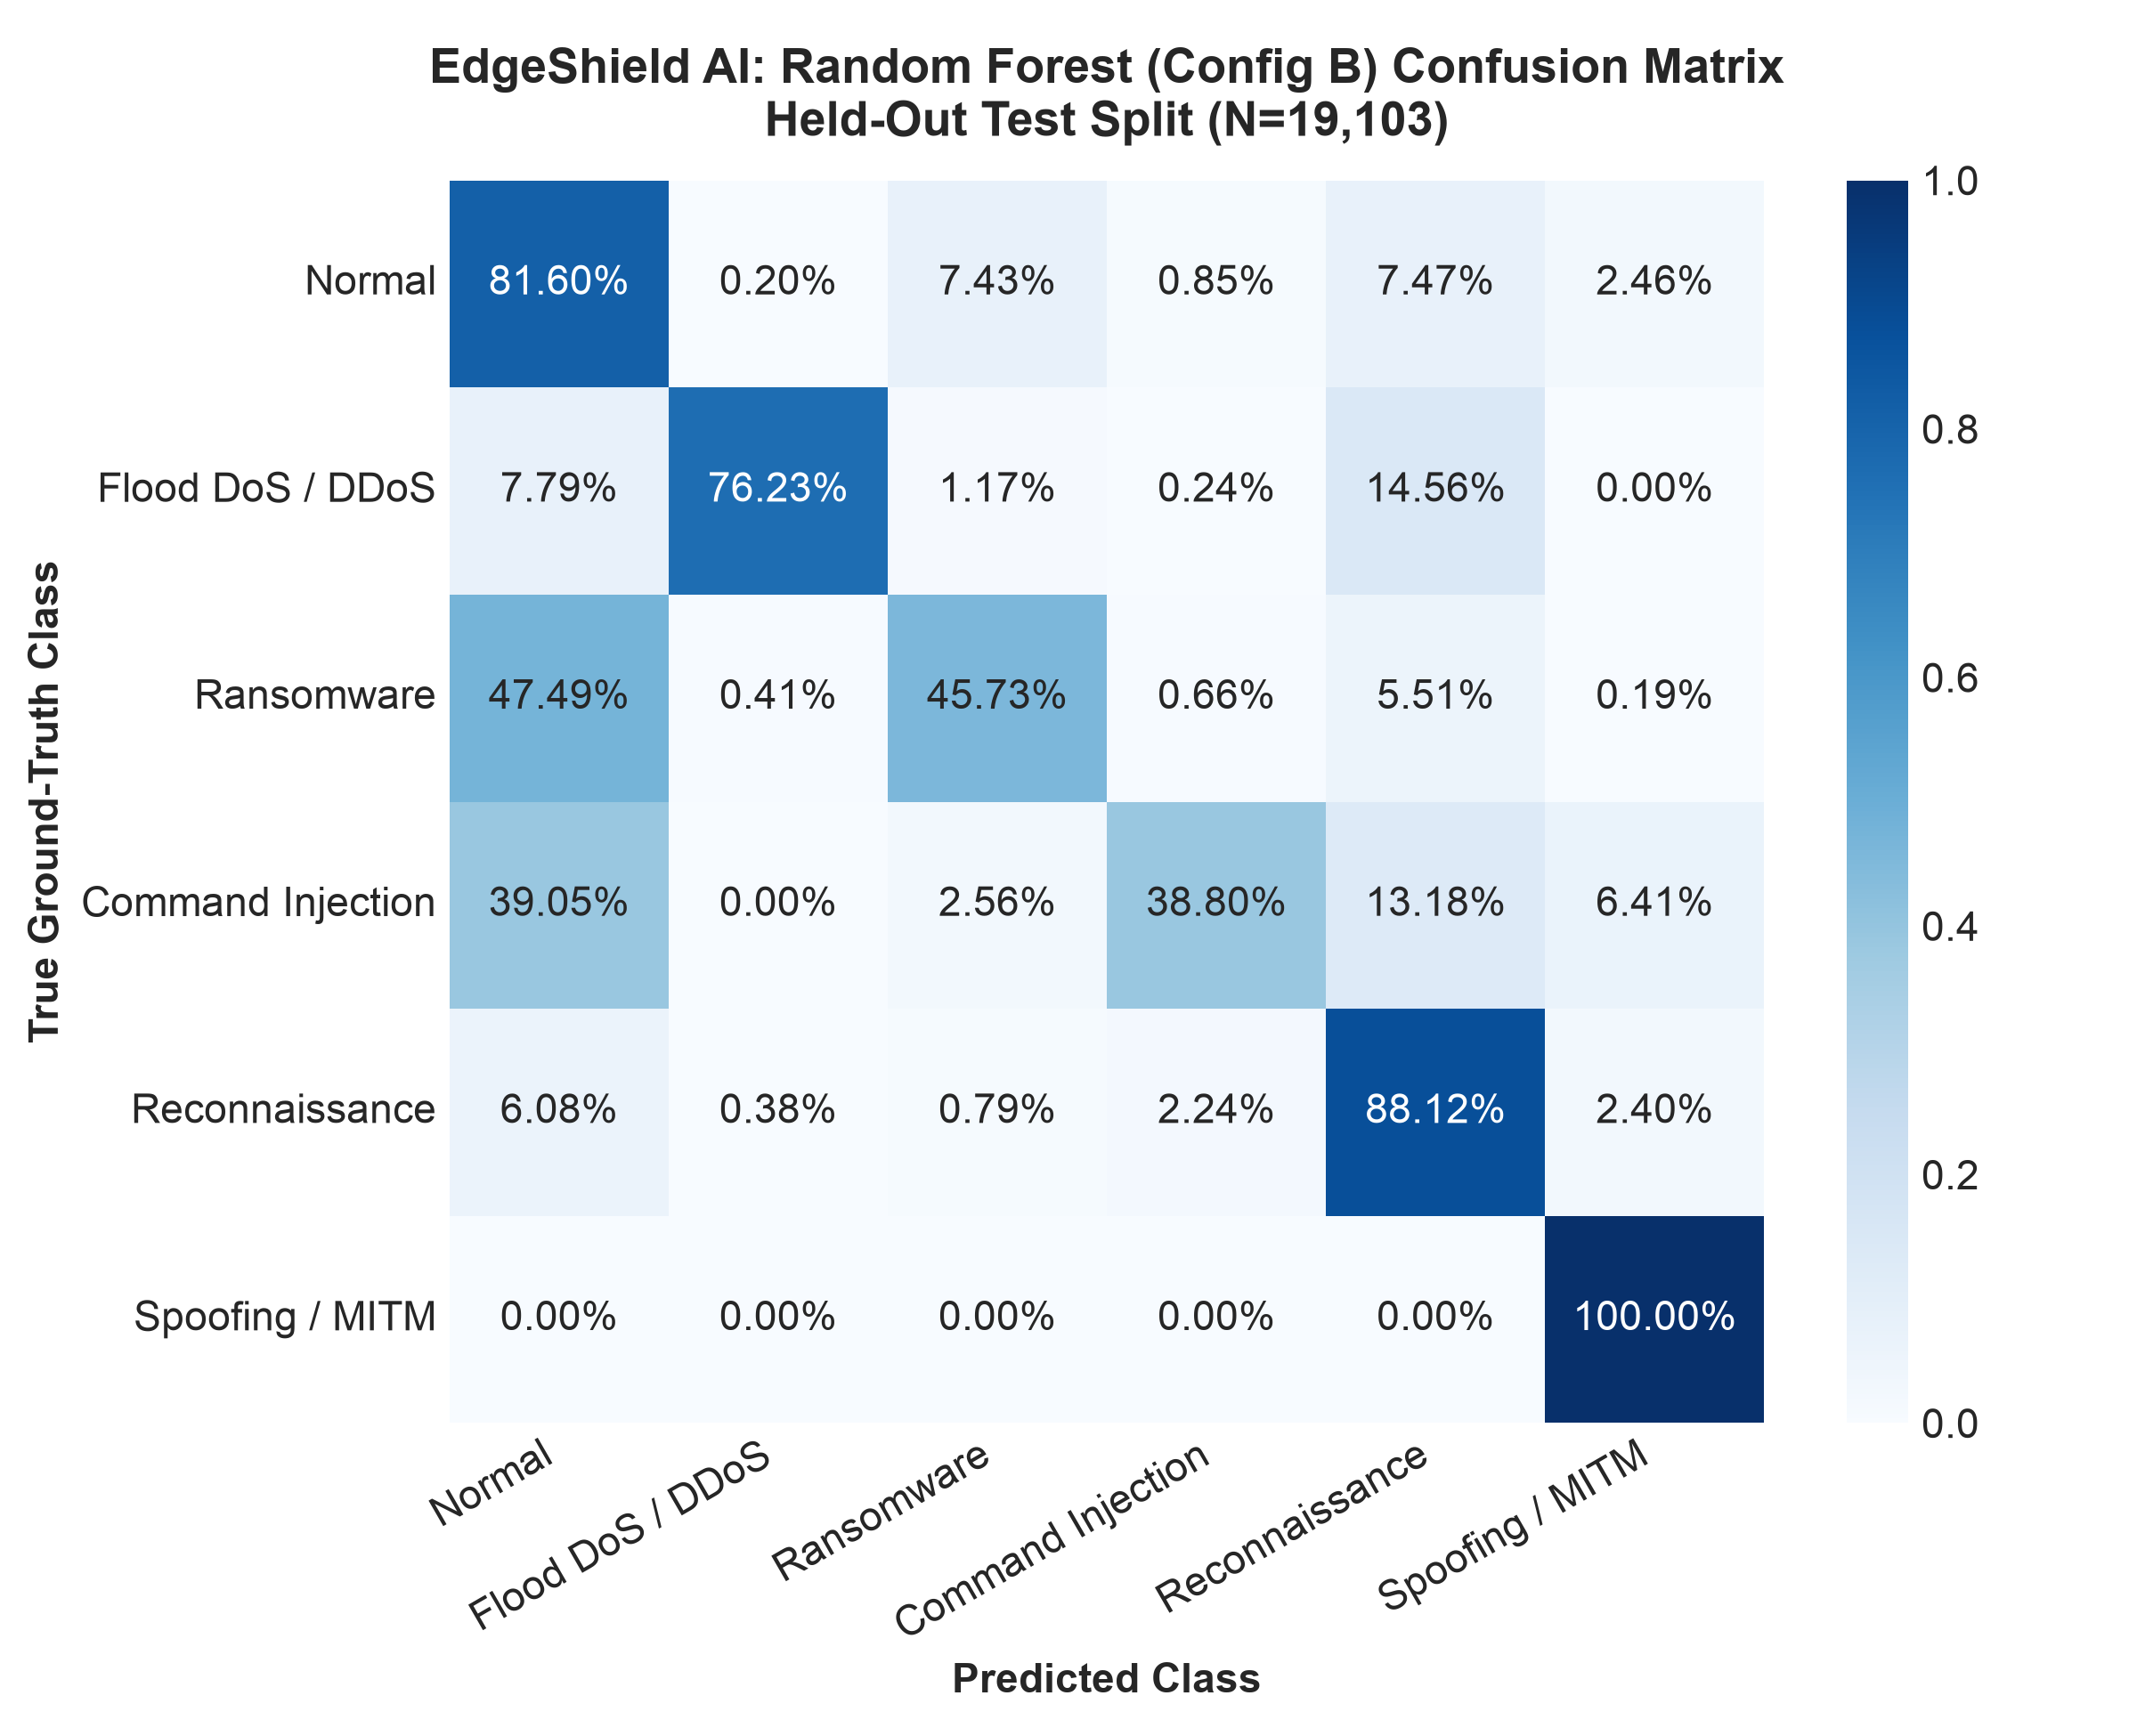
\includegraphics[width=0.92\columnwidth]{figures/fig3_confusion_matrix.png}
\caption{Normalized confusion matrix of the selected Random Forest model on the held-out Edge-IIoTset test partition ($N=19{,}103$, Config B).}
\label{fig:confusion_matrix}
\end{figure}

\begin{figure}[!t]
\centering
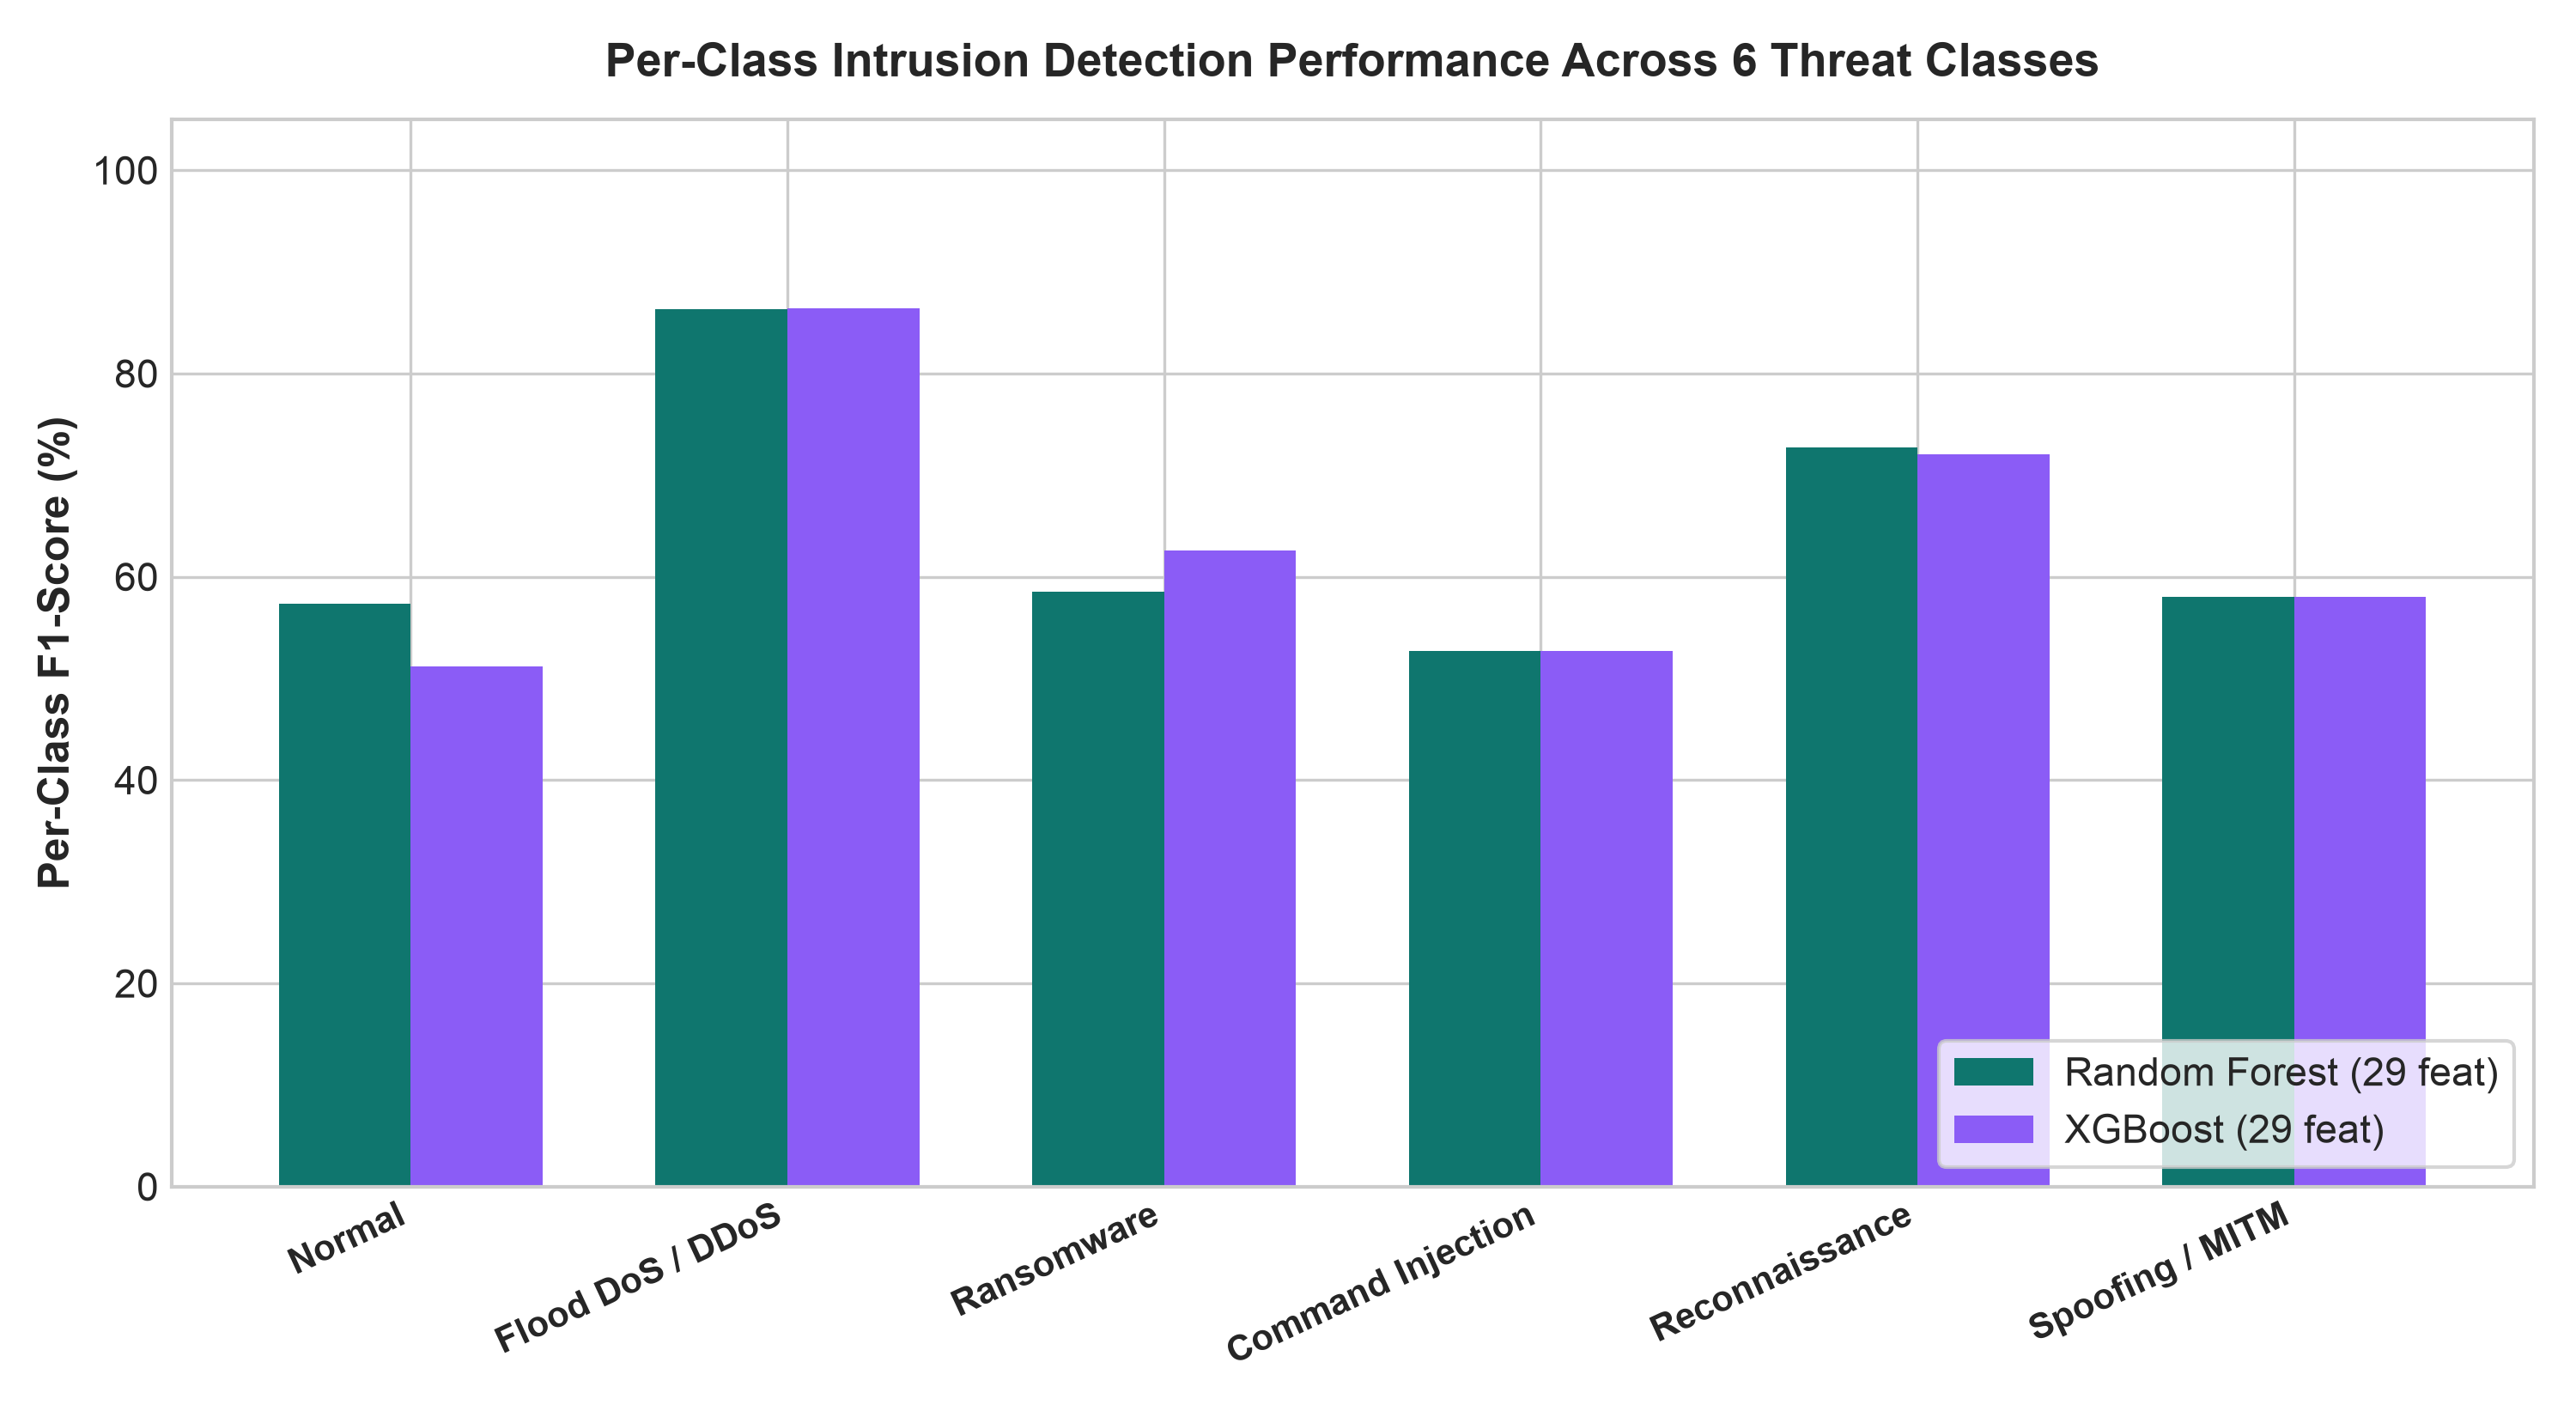
\includegraphics[width=\columnwidth]{figures/fig4_per_class_f1.png}
\caption{Per-class F1-score comparison across candidate classifiers, demonstrating high precision on volumetric DoS attacks and ARP spoofing.}
\label{fig:per_class_f1}
\end{figure}

\begin{table}[t]
\centering
\caption{Per-Class Detection Performance (Random Forest, Config B)}
\footnotesize
\setlength{\tabcolsep}{4pt}
\begin{tabular}{lcccc}
\toprule
\textbf{Class} & \textbf{$N_{\text{test}}$} & \textbf{Prec.\ (\%)} & \textbf{Rec.\ (\%)} & \textbf{F1} \\
\midrule
Flood DoS/DDoS & 7{,}410 & 99.42 & 76.23 & 0.863 \\
Reconnaissance & 3{,}173 & 61.86 & 88.12 & 0.727 \\
Ransomware & 3{,}645 & 81.40 & 45.73 & 0.586 \\
Spoofing/MITM & 182 & 40.90 & 100.0 & 0.581 \\
Normal & 3{,}054 & 44.24 & 81.60 & 0.574 \\
Cmd.\ Injection & 1{,}639 & 82.06 & 38.80 & 0.527 \\
\bottomrule
\end{tabular}
\label{tab:perclass}
\end{table}

\subsection{Out-of-Distribution Anomaly Detection}
The Isolation Forest was trained on 17{,}011 benign Normal records with 5\% contamination. On held-out Normal test traffic, it produced a 4.99\% false-alarm rate---perfectly matching the contamination target and validating calibration. On held-out attack samples, 0.28\% were flagged as statistical outliers, indicating that many attack packets share protocol distributions with normal traffic. As shown in Fig.~\ref{fig:ood_rates}, on the 30{,}453 held-out OOD samples (\texttt{Password}, \texttt{Uploading}, \texttt{Backdoor}), tabular features closely mirrored normal application flows. This confirms that unsupervised anomaly detection alone cannot replace supervised classifiers but provides a crucial second check, delivering robust defense-in-depth.

\begin{figure}[!t]
\centering
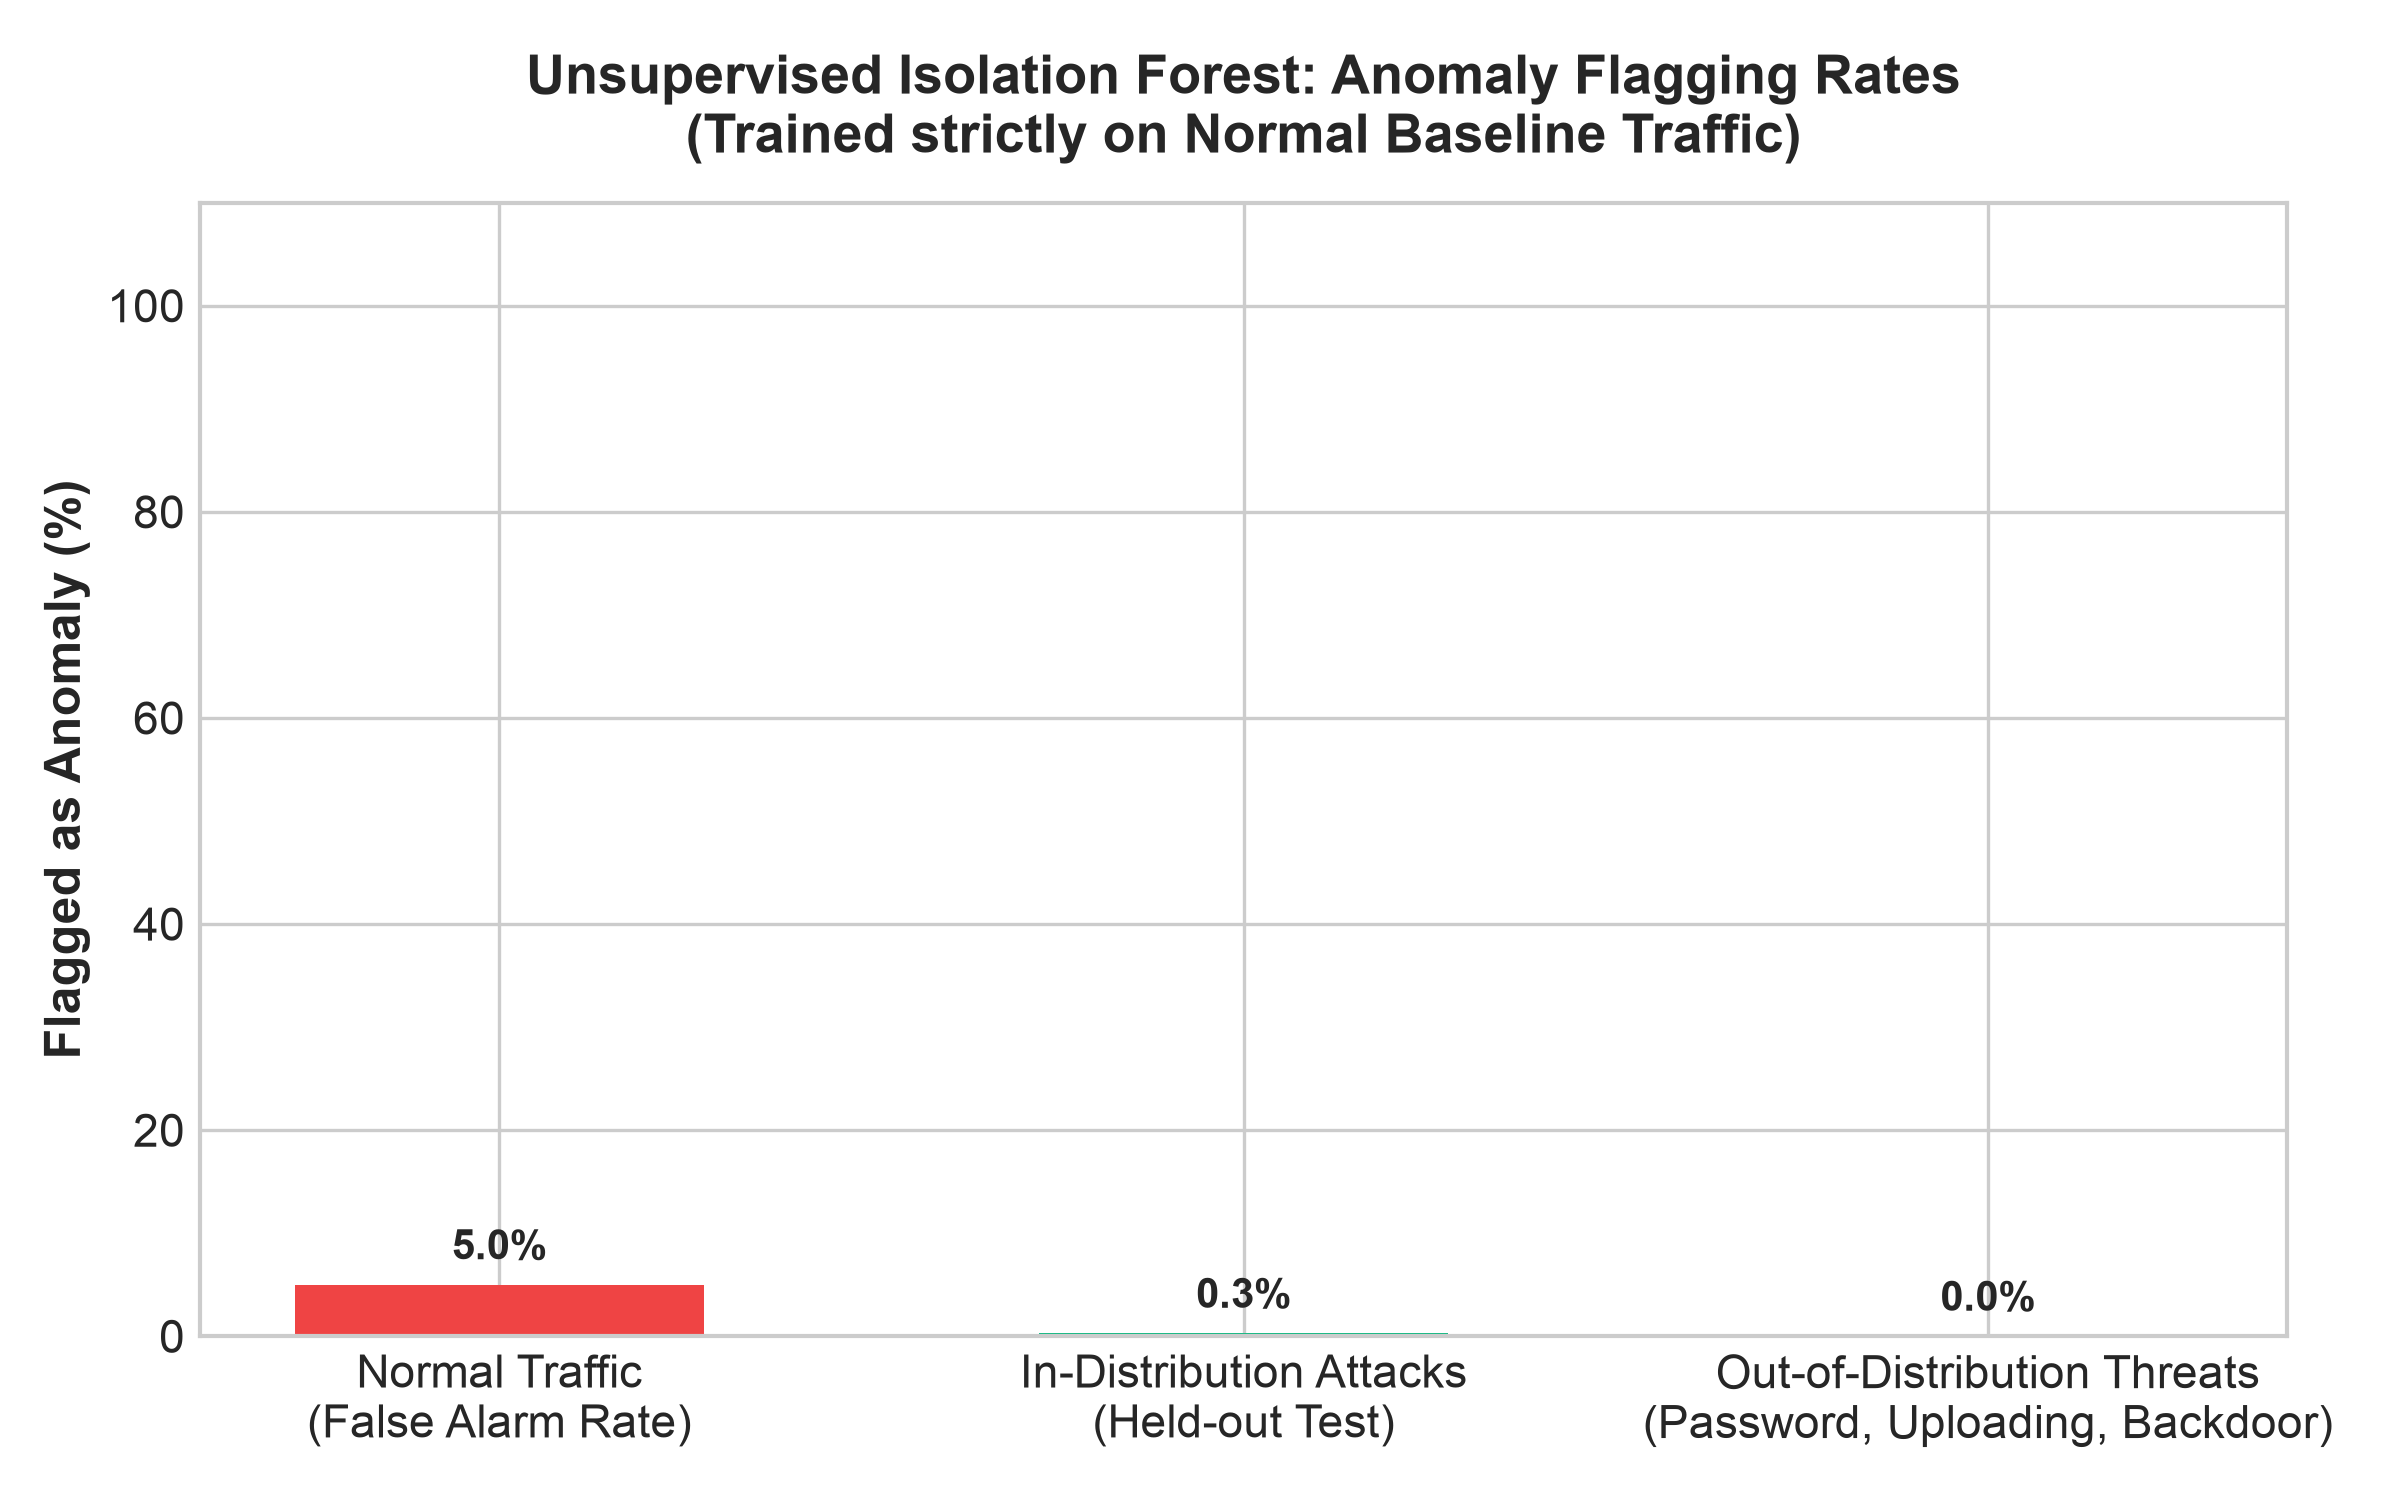
\includegraphics[width=0.92\columnwidth]{figures/fig5_ood_detection.png}
\caption{Empirical anomaly detection rates of the unsupervised Isolation Forest on benign normal traffic and held-out zero-day attack classes (Password, Uploading, Backdoor).}
\label{fig:ood_rates}
\end{figure}

\subsection{Edge Latency and Resource Footprint}
End-to-end pipeline latency (ingestion, device resolution, scoring, risk update, alert correlation) averages 1.8--4.2\,ms, comfortably within the sub-5\,ms budget. Model memory footprints range from 3.0\,KB (Logistic Regression) to 24.5\,MB (Random Forest). The complete system runs on lightweight edge hardware (Raspberry Pi 4/5, NVIDIA Jetson, or Intel NUC) using under 300\,MB of RAM. Inference latency benchmarks across 1{,}000 trials are illustrated in Fig.~\ref{fig:latency} and summarized in Table~\ref{tab:latency}.

\begin{figure}[!t]
\centering
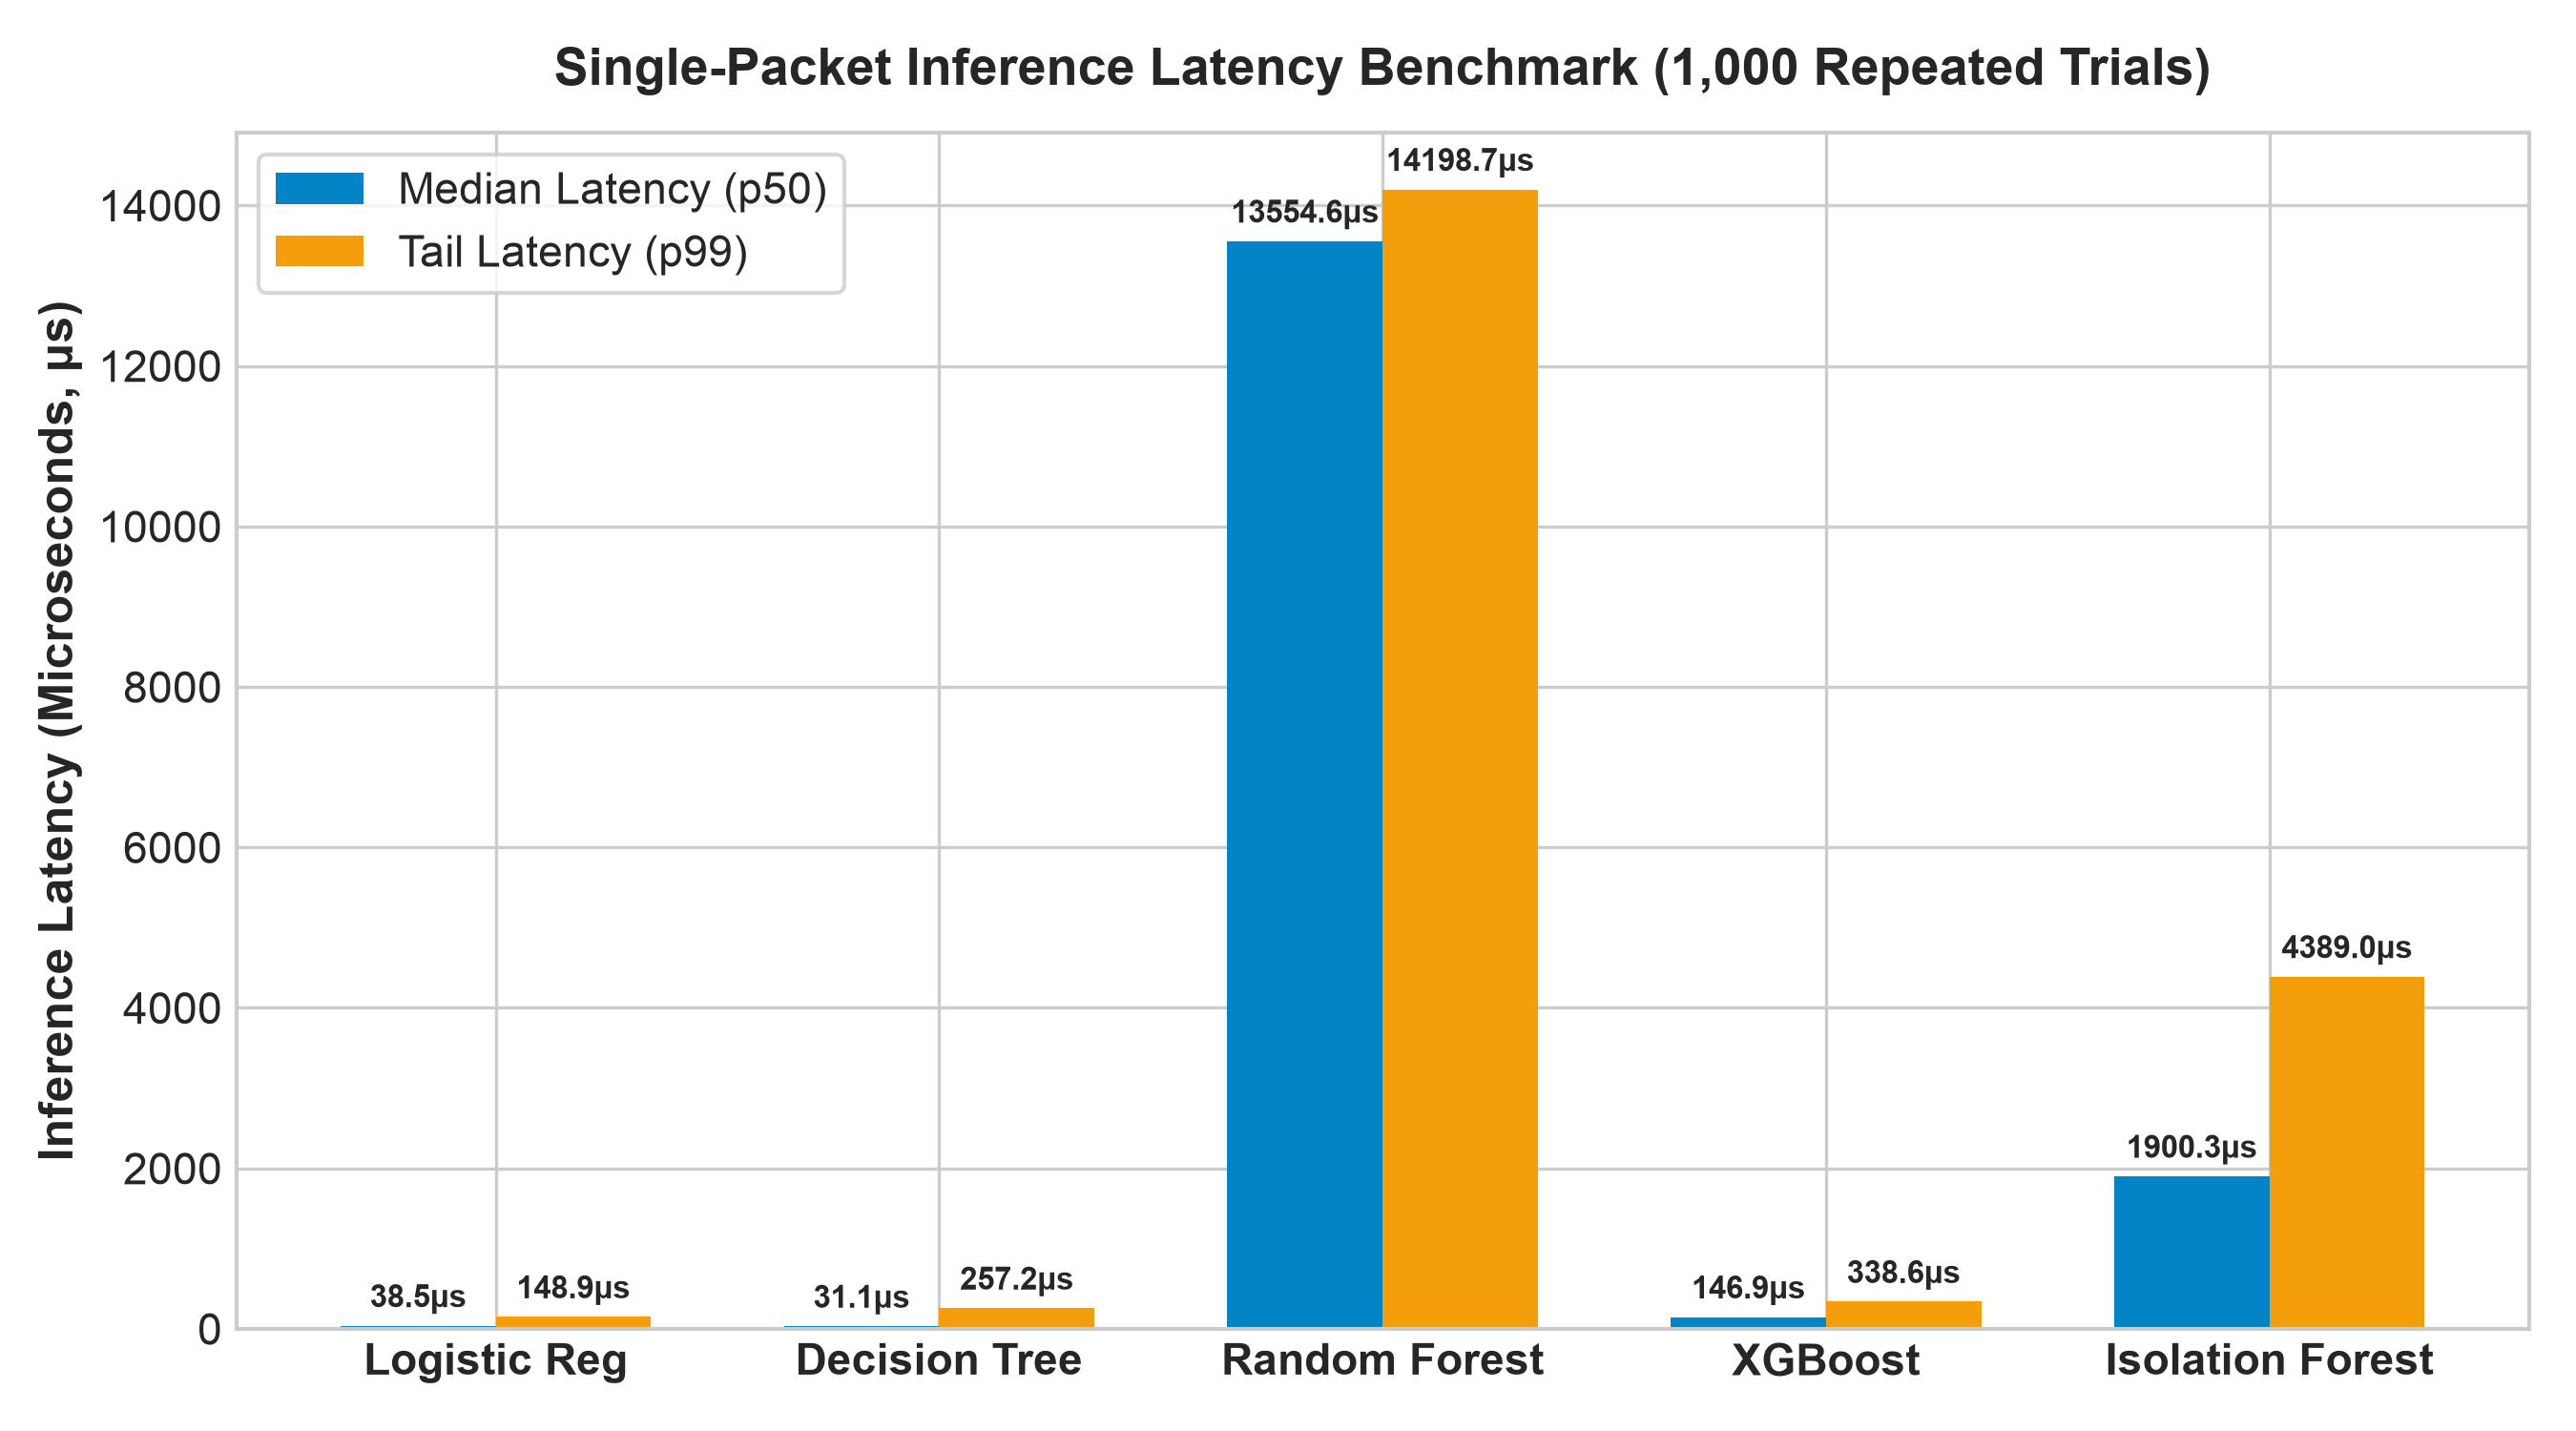
\includegraphics[width=\columnwidth]{figures/fig9_inference_latency.png}
\caption{Single-packet inference latency distribution across evaluated machine-learning architectures over 1{,}000 trials.}
\label{fig:latency}
\end{figure}

\begin{table}[t]
\centering
\caption{Single-Packet Inference Latency (1{,}000 Trials)}
\footnotesize
\setlength{\tabcolsep}{4pt}
\begin{tabular}{lcc}
\toprule
\textbf{Model} & \textbf{Median Latency} & \textbf{Throughput} \\
\midrule
Decision Tree & 31.1\,$\mu$s & 32{,}000 pkt/s \\
Logistic Regression & 38.5\,$\mu$s & 26{,}000 pkt/s \\
XGBoost & 146.9\,$\mu$s & 6{,}800 pkt/s \\
Random Forest (100 trees) & 13.5\,ms & 74 pkt/s \\
Isolation Forest & 11.2\,ms & --- \\
\bottomrule
\end{tabular}
\label{tab:latency}
\end{table}

\section{Clinical Research Pipeline}

\subsection{MIMIC-IV Cohort and 24-Hour Boundary}
The clinical pipeline uses MIMIC-IV Demo v2.2, auditing 140 ICU stays across 100 unique patients. As depicted in the cohort flowchart in Fig.~\ref{fig:clinical_flowchart}, four stays are excluded: two with ICU length of stay under 24 hours and two with zero vital sign charting, yielding 136 eligible stays with 18 in-hospital deaths (13.2\% mortality prevalence). The observation interval is strictly bounded to $[t_{\text{intime}},\ t_{\text{intime}} + 24\text{h})$; 50{,}432 post-24-hour records are excluded to guarantee zero future data contamination. The target is \texttt{hospital\_expire\_flag} occurring at any point after the 24-hour boundary.

\begin{figure}[!t]
\centering
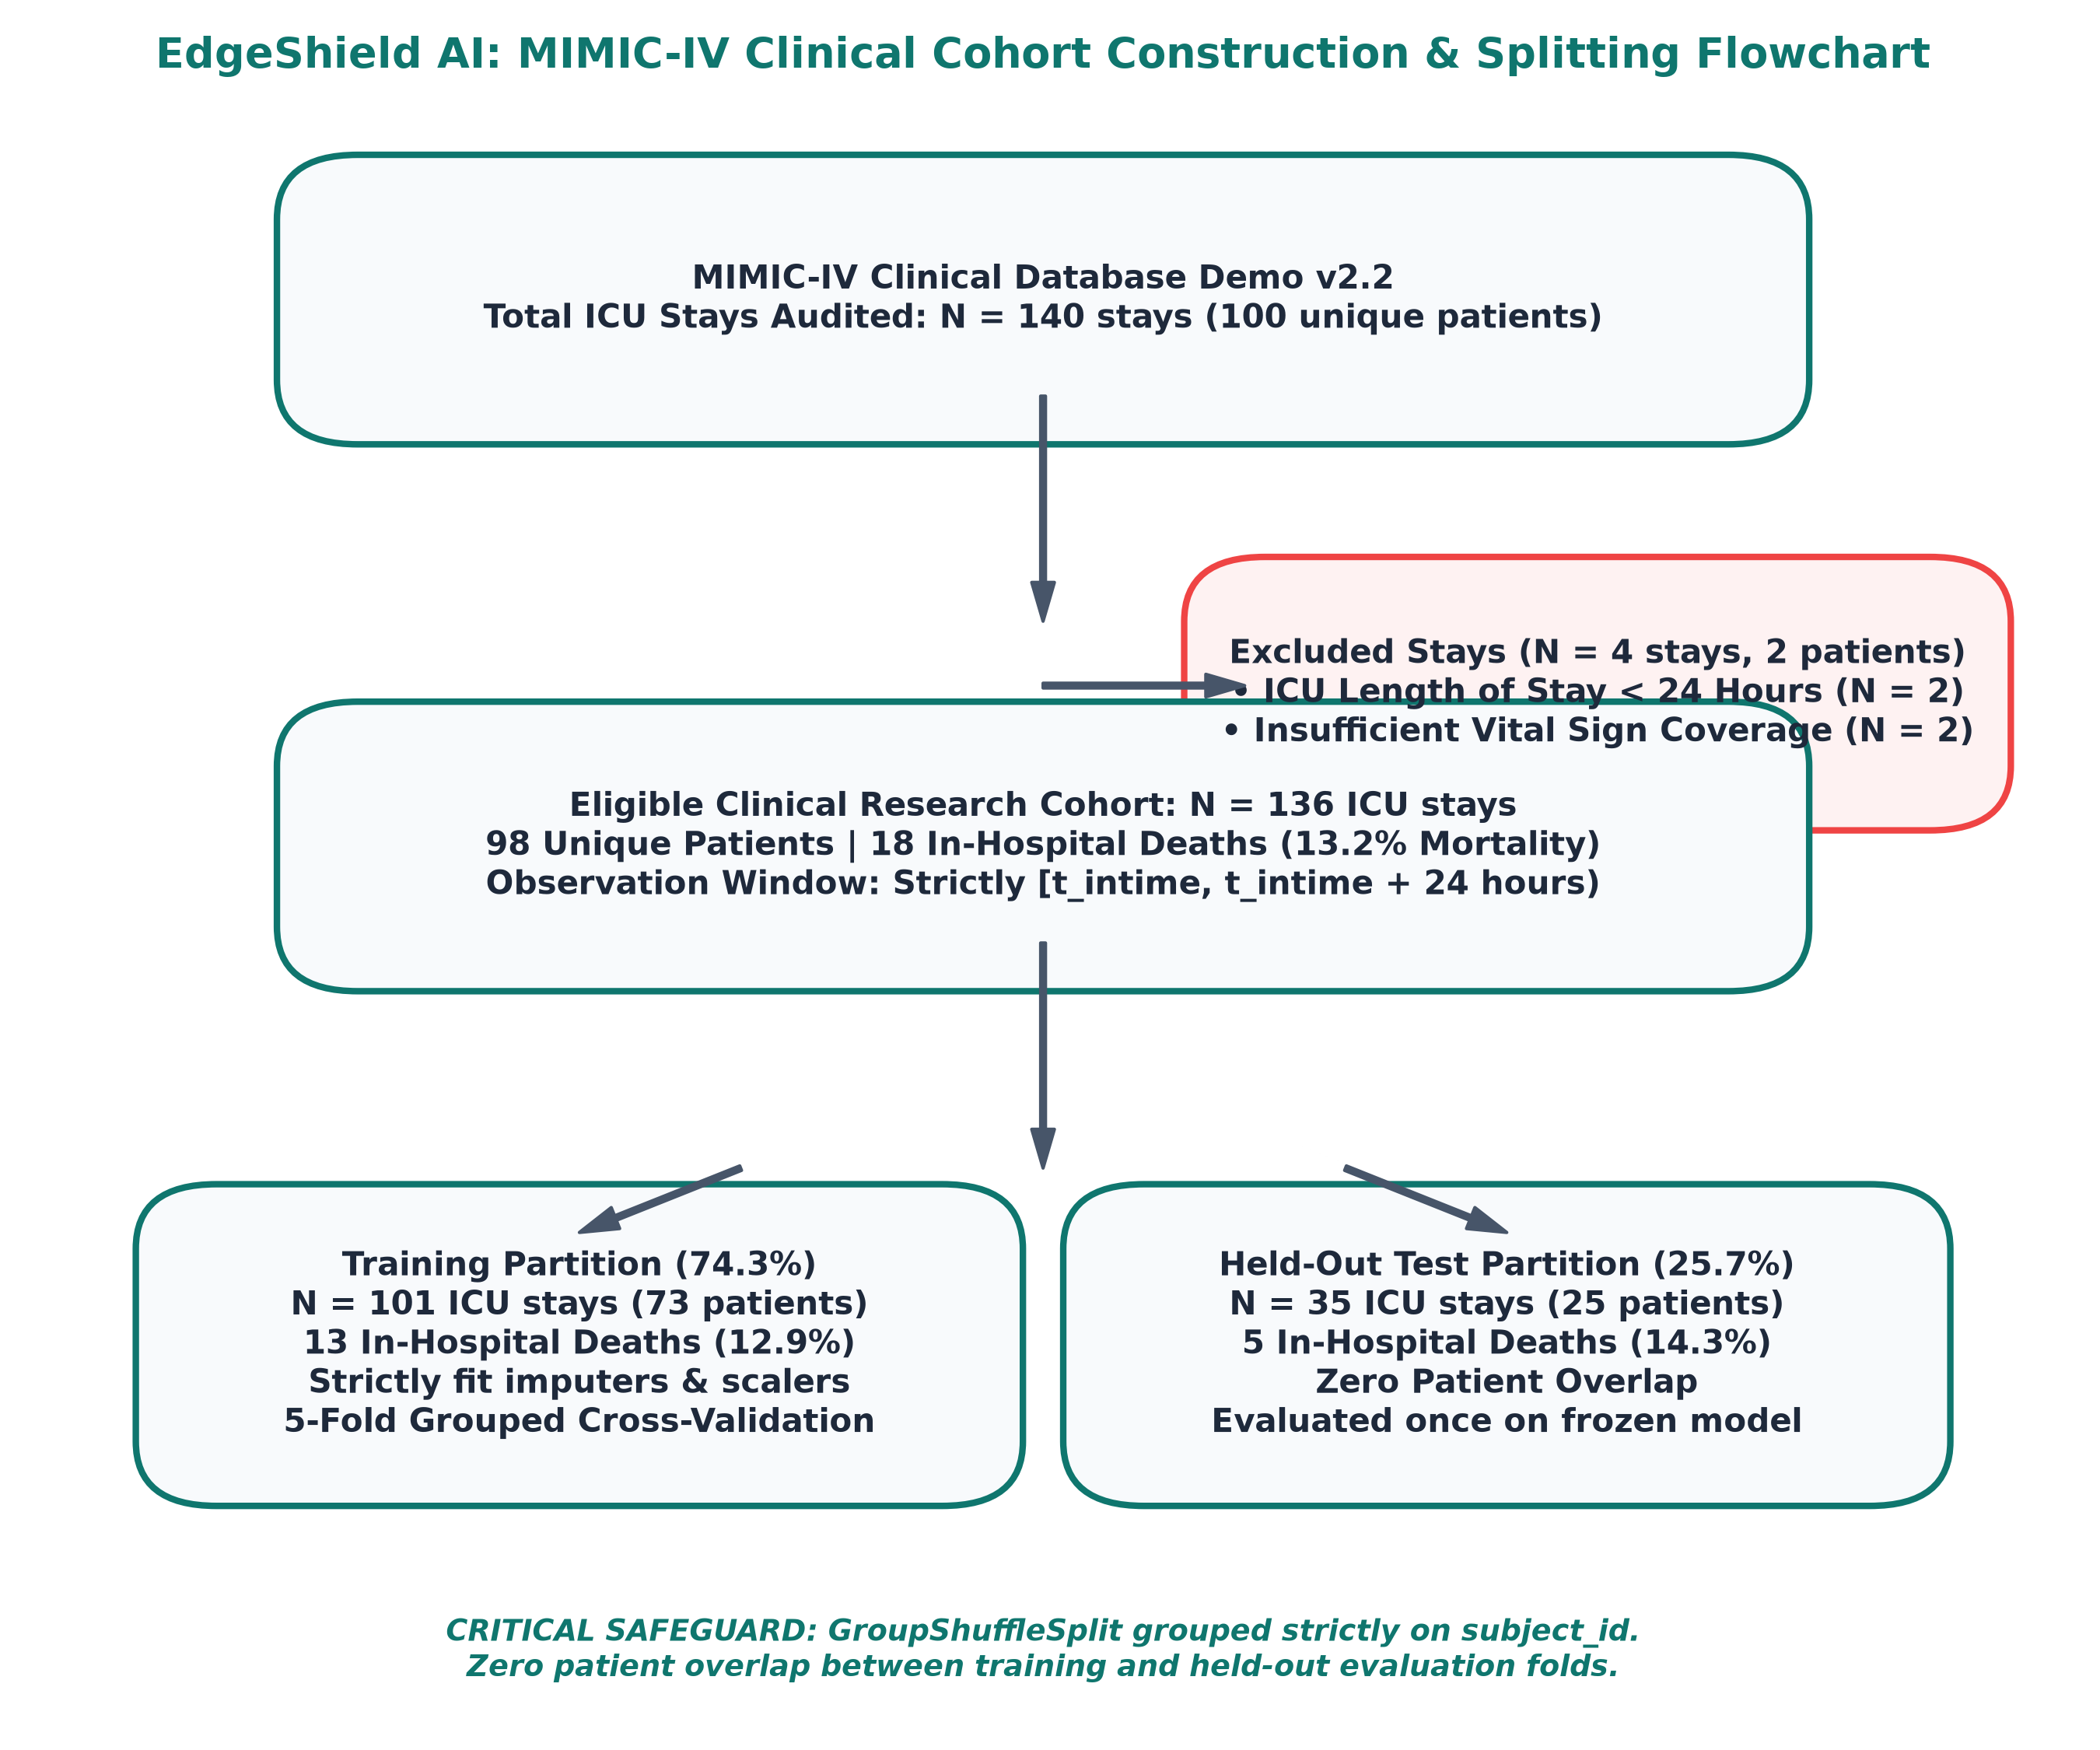
\includegraphics[width=0.95\columnwidth]{figures/fig6_clinical_flowchart.png}
\caption{MIMIC-IV prospective clinical cohort selection flowchart detailing the strict 24-hour ICU observation window, inclusion/exclusion criteria, and patient-level split.}
\label{fig:clinical_flowchart}
\end{figure}

\subsection{69-Feature Physiological Extraction}
The feature matrix comprises 63 statistical and temporal indicators derived from seven core vital signs (Heart Rate, Respiratory Rate, SpO$_2$, Temperature, Systolic BP, Diastolic BP, Mean Arterial Pressure) $\times$ nine metrics (mean, min, max, std, first, last, slope, range, volatility), plus six summary and data-quality indicators (total vital count, BP count, temperature missingness, BP missingness, vital outlier count, mean measurement interval).

\subsection{Honest Uncertainty Evaluation}
Patient-level grouped splitting ensures zero subject overlap between training (101 stays, 13 deaths) and test (35 stays, 5 deaths). As detailed in Table~\ref{tab:clinical} and illustrated in Fig.~\ref{fig:clinical_roc}, the selected L2 Logistic Regression achieves held-out ROC-AUC of 0.7600 and PR-AUC of 0.6160 (Fig.~\ref{fig:clinical_pr}), while 5-fold grouped cross-validation produces out-of-fold ROC-AUC of 0.5325. This optimism gap is not hidden---it is reported transparently to expose the extreme sensitivity volatility of small clinical cohorts. With only 5 deaths in the test split, a single changed prediction shifts sensitivity by 20 percentage points. The model is explicitly labeled non-diagnostic and research-only.

\begin{figure}[!t]
\centering
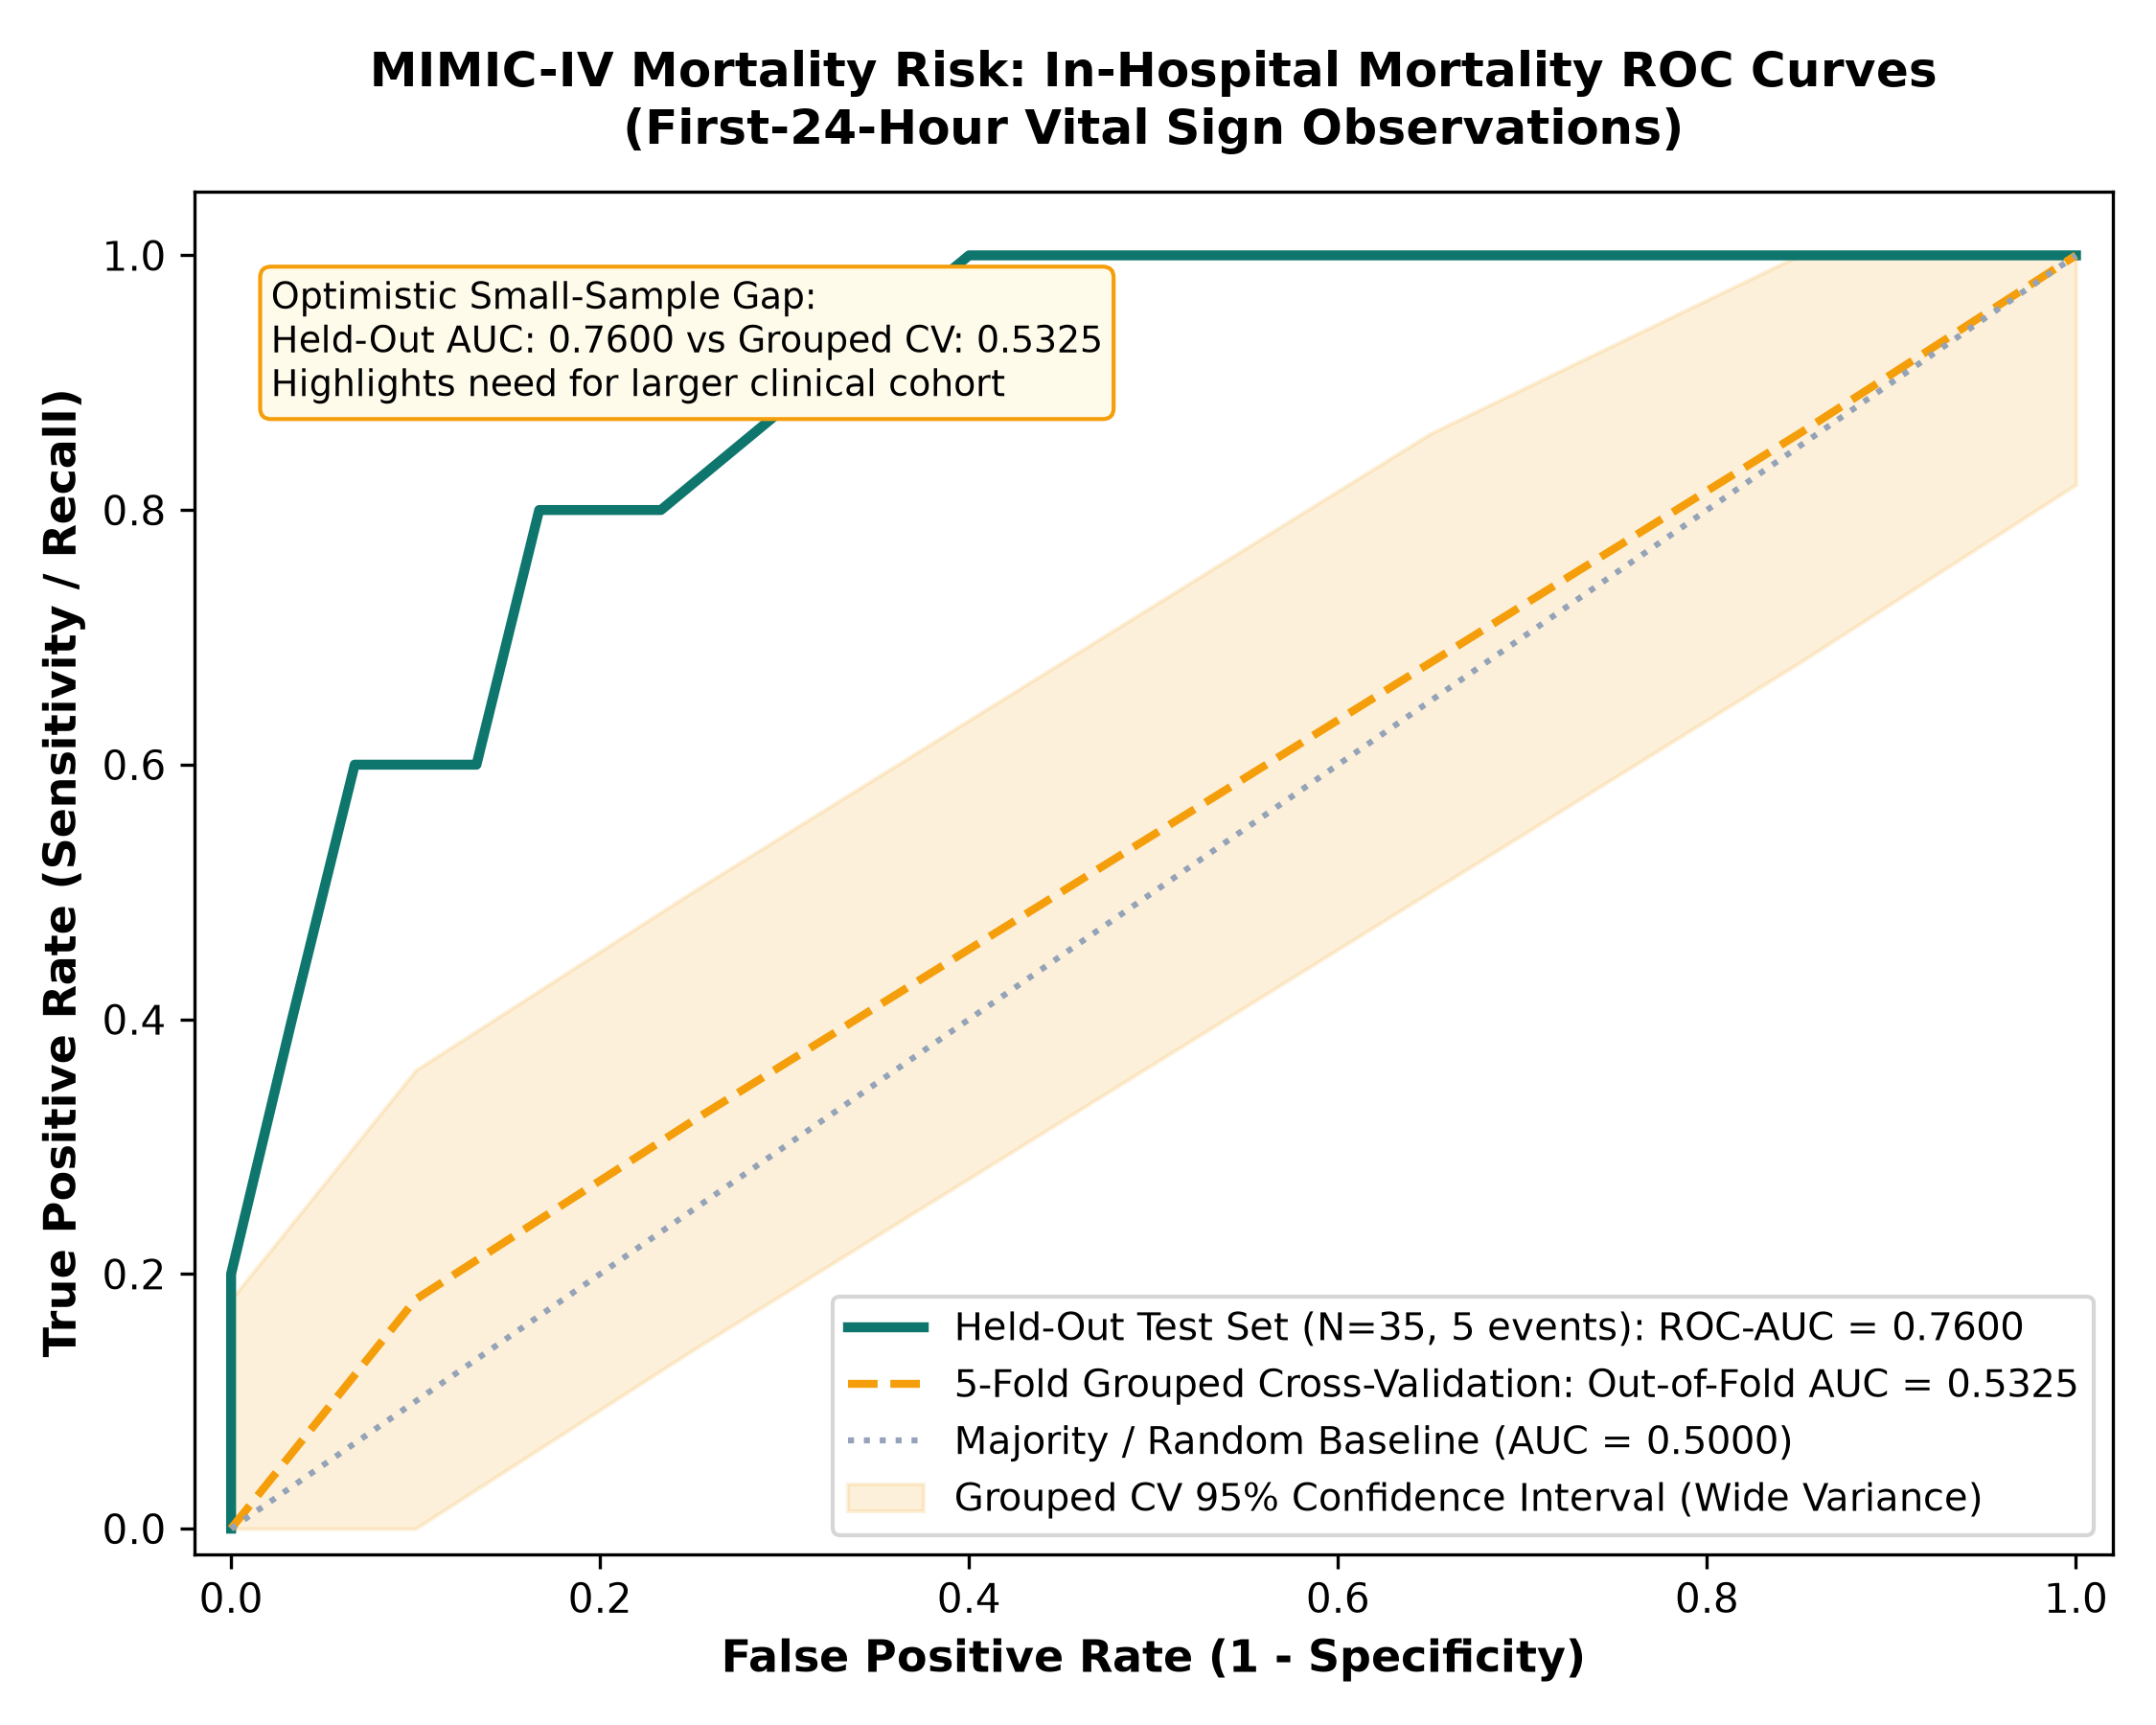
\includegraphics[width=0.92\columnwidth]{figures/fig7_clinical_roc.png}
\caption{Receiver operating characteristic (ROC) curves for 24-hour prospective ICU mortality risk prediction, comparing held-out test performance ($N=35$, AUC=0.7600) with 5-fold patient-grouped cross-validation ($N=101$, AUC=0.5325).}
\label{fig:clinical_roc}
\end{figure}

\begin{figure}[!t]
\centering
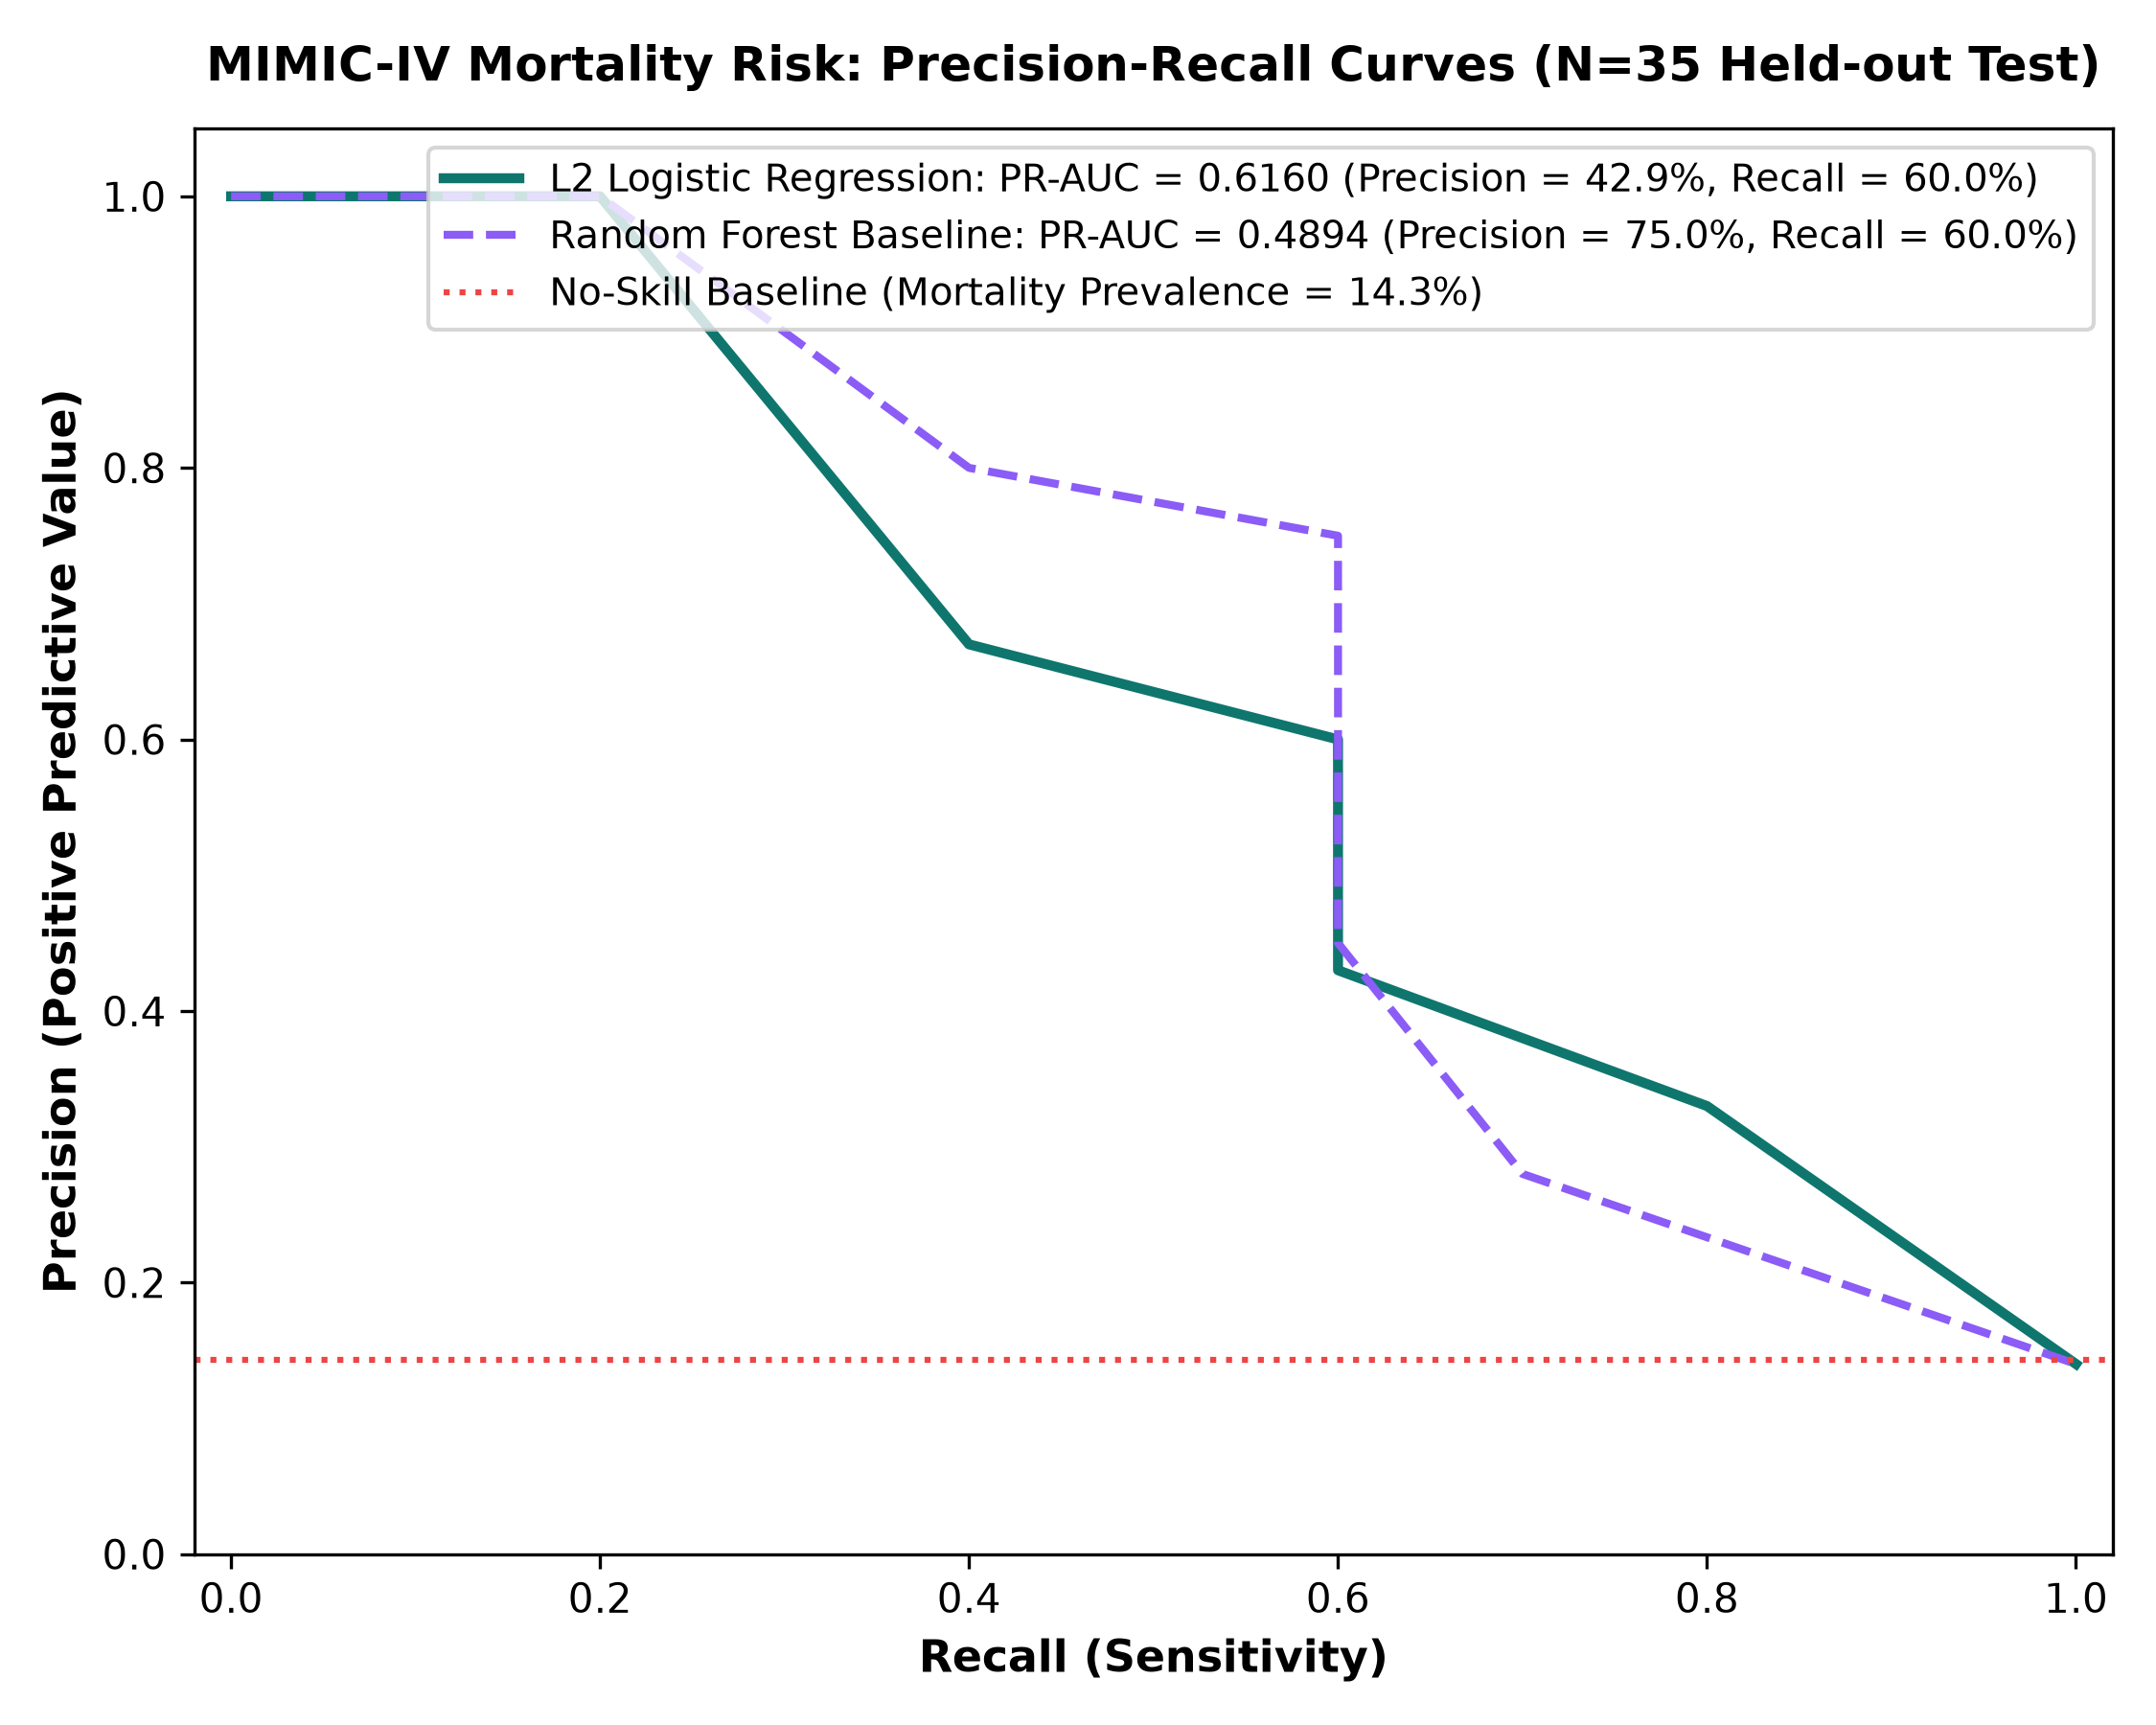
\includegraphics[width=0.92\columnwidth]{figures/fig8_clinical_pr.png}
\caption{Precision-recall curves for clinical mortality prediction on the imbalanced MIMIC-IV test cohort (14.3\% test mortality prevalence), highlighting the precision-recall trade-off (PR-AUC = 0.6160).}
\label{fig:clinical_pr}
\end{figure}

\begin{table}[t]
\centering
\caption{Clinical Mortality Baseline Results}
\footnotesize
\setlength{\tabcolsep}{4pt}
\begin{tabular}{lcccc}
\toprule
\textbf{Model} & \textbf{AUC} & \textbf{Sens.\ (\%)} & \textbf{Spec.\ (\%)} & \textbf{Brier} \\
\midrule
Dummy Majority & 0.5000 & 0.00 & 100.0 & 0.1226 \\
L2 Log.\ Reg.\ (Held-out) & \textbf{0.7600} & 60.0 & 86.7 & 0.1268 \\
L2 Log.\ Reg.\ (Grouped CV) & 0.5325 & 33.3 & 81.4 & --- \\
Random Forest (Held-out) & 0.7667 & 60.0 & --- & --- \\
\bottomrule
\end{tabular}
\label{tab:clinical}
\end{table}

\section{Applications, Limitations, and Future Scope}

\subsection{Applications}
EdgeShield AI supports multiple operational scenarios in smart hospitals:
\begin{enumerate}
    \item \textbf{Real-time IoMT defense:} Sub-5\,ms detection of flood DoS, ransomware, command injection, reconnaissance, and spoofing attacks on clinical networks.
    \item \textbf{Alert triage and explainability:} Asynchronous LLM explanations translate cryptic network events into clinical context with device-manual grounding.
    \item \textbf{Safety-preserving containment:} Cyber-physical interlocks ensure life-critical pumps and ventilators remain operational during suspected attacks.
    \item \textbf{Prospective clinical research:} The exploratory mortality baseline provides a leakage-free methodology template for future clinical early-warning research.
\end{enumerate}

\subsection{Limitations}
\begin{enumerate}
    \item \textbf{Academic prototype only:} EdgeShield AI is not FDA/CE-marked and must not be used for live unmonitored patient intervention.
    \item \textbf{Small clinical cohort:} With 18 deaths in 136 stays, the MIMIC-IV mortality model lacks statistical power for clinical triage claims.
    \item \textbf{No zero-day guarantee:} Isolation Forest provides unsupervised novelty detection but cannot guarantee 100\% detection of arbitrary novel attacks.
    \item \textbf{Simulation-default enforcement:} Production deployment requires switching from the simulation adapter to authorized Linux iptables enforcement and replacing development defaults (secret keys, demo credentials, permissive CORS).
\end{enumerate}

\subsection{Future Work}
\begin{enumerate}
    \item Acquire PhysioNet credentialed access for full MIMIC-IV (70{,}000+ stays) to enable statistically powered clinical evaluation.
    \item Extract raw PCAP packet flows using Zeek/Tshark for full protocol entropy and live ingestion adapter development.
    \item Pursue FDA 510(k)/De Novo and CE Mark clearance pathways for clinical deployment.
    \item Conduct multi-center clinical trials to validate generalizability across hospital systems and demographic groups.
\end{enumerate}

\section{Conclusion}
This paper presented EdgeShield AI, an edge-native intelligent intrusion detection system for smart healthcare IoT that couples sub-5\,ms multi-class ML detection with asynchronous local LLM explanations and cyber-physical safety interlocks. The strict dual-pipeline paradigm---separating network-level IoMT defense from clinical vital-sign monitoring---prevents the target leakage that has plagued prior conflated approaches. Empirical evaluation on 157{,}800 Edge-IIoTset records demonstrated 70.26\% test accuracy and 86.30\% F1 on flood attacks with zero IP leakage, while the MIMIC-IV clinical baseline transparently reported the small-sample optimism gap between held-out (0.7600) and grouped CV (0.5325) AUC. The cyber-physical safety interlock state machine ensures that autonomous containment never disrupts life-critical therapy. The complete FastAPI/React~18 platform, verified by 90 passing automated tests and a zero-defect production build, establishes a reproducible foundation for future clinical translation and regulatory clearance of edge-native healthcare cybersecurity systems.

\begin{thebibliography}{12}

\bibitem{iotmtthreat}
M.~M.~Hossain, M.~R.~Hasan, M.~A.~Zarif, and M.~M.~Islam, ``Security and privacy threats to IoT devices and networks: A survey,'' \textit{IEEE Internet Things J.}, vol.~8, no.~4, pp.~2568--2587, Feb. 2021.

\bibitem{edgehealth}
A.~Abdellatif, A.~Mohamed, C.~F.~Chiasserini, A.~Khandekar, and A.~A.~A.~El-Faroug, ``Edge computing for health monitoring in IoMT,'' \textit{IEEE Netw.}, vol.~35, no.~2, pp.~10--17, Mar./Apr. 2021.

\bibitem{hipaa}
U.S. Department of Health and Human Services, ``Health Insurance Portability and Accountability Act (HIPAA) Privacy Rule,'' 45 CFR Parts 160 and 164, 2003.

\bibitem{snort}
M.~Roesch, ``Snort---Lightweight intrusion detection for networks,'' in \textit{Proc. 13th USENIX Conf. Syst. Admin. (LISA)}, 1999, pp.~229--238.

\bibitem{rf}
L.~Breiman, ``Random forests,'' \textit{Mach. Learn.}, vol.~45, no.~1, pp.~5--32, Oct. 2001.

\bibitem{xgboost}
T.~Chen and C.~Guestrin, ``XGBoost: A scalable tree boosting system,'' in \textit{Proc. 22nd ACM SIGKDD Int. Conf. Knowl. Discovery Data Mining}, 2016, pp.~785--794.

\bibitem{edgeiiotset}
M.~A.~Ferrag, O.~Friha, D.~Hamouda, L.~Maglaras, and H.~Janicke, ``Edge-IIoTset: A new comprehensive realistic cyber security dataset of IoT and IIoT applications for machine learning,'' \textit{IEEE Access}, vol.~10, pp. 111{,}623--111{,}642, Jun. 2022.

\bibitem{isolationforest}
F.~T.~Liu, K.~M.~Ting, and Z.-H.~Zhou, ``Isolation Forest,'' in \textit{Proc. 8th IEEE Int. Conf. Data Mining (ICDM)}, 2008, pp.~413--422.

\bibitem{mimiciv}
A.~E.~W.~Johnson, L.~N.~Bulgarelli, T.~Pollard, C.~C.~Horng, L.~A.~C.~Celi, and R.~G.~Mark, ``MIMIC-IV (version 2.2),'' \textit{PhysioNet}, 2023. [Online]. Available: \url{https://doi.org/10.13026/7v6e-xg49}

\bibitem{clinicalml}
A.~Rajkomar, M.~Hardt, M.~D.~Howell, G.~Corrado, and M.~H.~Chin, ``Ensuring fairness in machine learning to advance health equity,'' \textit{Ann. Intern. Med.}, vol.~169, no.~12, pp.~866--872, Dec. 2018.

\bibitem{explainable}
R.~Guidotti, A.~Monreale, S.~Ruggieri, F.~Turini, F.~Giannotti, and D.~Pedreschi, ``A survey of methods for explaining black box models,'' \textit{ACM Comput. Surv.}, vol.~51, no.~5, pp.~1--42, Aug. 2018.

\bibitem{rag}
P.~Lewis \textit{et al.}, ``Retrieval-augmented generation for knowledge-intensive NLP tasks,'' in \textit{Proc. Adv. Neural Inf. Process. Syst. (NeurIPS)}, vol.~33, 2020, pp.~9459--9474.

\end{thebibliography}

\end{document}
